\chapter{Implementation}
\label{implementation}

In this chapter we are going to be more specific about the details of our implementation that we produced from our design. At first, we will state our virtual network function (\acrshort{vnf}) specifications, before describing some details about our components, the realization of our previously mentioned concepts and challenges we faced while implementing.


\section{Specification}
\label{impl_specification}
In this section we will focus on our specifications. First we will present our protocol specifications for each \acrshort{vnf}, before providing communication examples to create and remove a slice.

\subsection{OpenAPI specifications}
To interconnect our \acrshort{vnf}s, we use multiple \acrshort{rest} \acrshort{api}s. Our \acrshort{rest} protocol specifications are conveniently provided via \Gls{openapi} descriptions \cite{openapi}. \Gls{openapi} is a project unifying the specification of web protocols by providing protocol descriptions in either JSON or YAML format. This way, our and future implementations of our protocols can auto-generate code to communicate with our services by using the \Gls{openapi} generator project \cite{openapi-generator}. \Gls{openapi} generators take a protocol description and convert them to something else. This can be client or server implementations written in various programming languages. There are also other projects providing support to present the specifications in human-readable form to developers, such as SwaggerUI \cite{swaggerui} or Redocly \cite{redocly}.

We provide \Gls{openapi} specifications for each service required by our design. The specifications can be found at the end of this thesis (see Appendix \ref{specifications}) in human-readable form, or in the accompanying sources in JSON format. We chose to unify the implementations of \acrshort{esmf} and \acrshort{ctmf}, as well as the implementations of \acrshort{dsmf} and \acrshort{dtmf} though, because their implementations are identical apart from enabling or disabling certain functionality.

The basic endpoints of each component can be seen in the tables \ref{table:esmf} through \ref{table:vpn_gateway}. Further details on parameters and responses can be found at the end of this thesis in Appendix \ref{specifications}.

All \acrshort{vnf}s provide endpoints for authentication (apart from the \acrshort{sdn} controller). This is currently just a placeholder to establish a real authentication scheme later. In the current specification the authentication endpoint takes no parameters and returns a predefined token. All the other endpoints then take this token to authorize requests. The details on how these endpoints work together can then be seen in Section \ref{impl_communication}, where we take a closer look on the creation and removal of a slice.

\begin{table}[htp]
    \begin{tabularx}{\textwidth}{ |l|X| }
        \hline
        \textbf{Endpoint}       & \textbf{Description}                                                                                \\
        \hline
        /v1/auth                & Endpoint that can be contacted by all parties to authenticate and obtain a new authentication token \\
        /v1/configuration       & Endpoint to configure this service                                                                  \\
        \hline
        /v1/slice               & Endpoint that can be contacted by hosts to submit new slice requests                                \\
        \hline
        /v1/slice\_reservation  & Endpoint used by other \acrshort{esmf}s to reserve a slice                                          \\
        /v1/slice\_deployment   & Endpoint used by other \acrshort{esmf}s to deploy a slice                                           \\
        /v1/tunnel\_reservation & Endpoint used by other \acrshort{esmf}s to reserve a tunnel                                         \\
        /v1/tunnel\_deployment  & Endpoint used by other \acrshort{esmf}s to deploy a tunnel                                          \\
        \hline
    \end{tabularx}
    \caption[\acrshort{esmf} endpoints]{The endpoints of our \acrshort{esmf} implementation alongside their functionality.}
    \label{table:esmf}
\end{table}

\begin{table}[htp]
    \begin{tabularx}{\textwidth}{ |l|X| }
        \hline
        \textbf{Endpoint}       & \textbf{Description}                                                                                \\
        \hline
        /v1/auth                & Endpoint that can be contacted by all parties to authenticate and obtain a new authentication token \\
        /v1/configuration       & Endpoint to configure this service                                                                  \\
        \hline
        /v1/tunnel\_reservation & Endpoint used by \acrshort{esmf}s to reserve a tunnel                                               \\
        /v1/tunnel\_deployment  & Endpoint used by \acrshort{esmf}s to deploy a tunnel                                                \\
        \hline
    \end{tabularx}
    \caption[\acrshort{ctmf} endpoints]{The endpoints of our \acrshort{ctmf} implementation alongside their functionality. Includes a subset of the \acrshort{esmf} endpoints.}
    \label{table:ctmf}
\end{table}

\begin{table}[htp]
    \begin{tabularx}{\textwidth}{ |l|X| }
        \hline
        \textbf{Endpoint}       & \textbf{Description}                                                                                \\
        \hline
        /v1/auth                & Endpoint that can be contacted by all parties to authenticate and obtain a new authentication token \\
        /v1/configuration       & Endpoint to configure this service                                                                  \\
        \hline
        /v1/slice\_reservation  & Endpoint used by our \acrshort{esmf} to reserve a slice                                             \\
        /v1/slice\_deployment   & Endpoint used by our \acrshort{esmf} to deploy a slice                                              \\
        /v1/tunnel\_reservation & Endpoint used by our \acrshort{esmf} to reserve a tunnel                                            \\
        /v1/tunnel\_deployment  & Endpoint used by our \acrshort{esmf} to deploy a tunnel                                             \\
        \hline
    \end{tabularx}
    \caption[\acrshort{dsmf} endpoints]{The endpoints of our \acrshort{dsmf} implementation alongside their functionality.}
    \label{table:dsmf}
\end{table}

\begin{table}[htp]
    \begin{tabularx}{\textwidth}{ |l|X| }
        \hline
        \textbf{Endpoint}       & \textbf{Description}                                                                                \\
        \hline
        /v1/auth                & Endpoint that can be contacted by all parties to authenticate and obtain a new authentication token \\
        /v1/configuration       & Endpoint to configure this service                                                                  \\
        \hline
        /v1/tunnel\_reservation & Endpoint used by our \acrshort{esmf} to reserve a tunnel                                            \\
        /v1/tunnel\_deployment  & Endpoint used by our \acrshort{esmf} to deploy a tunnel                                             \\
        \hline
    \end{tabularx}
    \caption[\acrshort{dtmf} endpoints]{The endpoints of our \acrshort{dtmf} implementation alongside their functionality. Includes a subset of the \acrshort{dsmf} endpoints.}
    \label{table:dtmf}
\end{table}

\begin{table}[htp]
    \begin{tabularx}{\textwidth}{ |l|X| }
        \hline
        \textbf{Endpoint} & \textbf{Description}                                                                                \\
        \hline
        /v1/auth          & Endpoint that can be contacted by all parties to authenticate and obtain a new authentication token \\
        \hline
        /v1/queue         & Endpoint used to manage \acrshort{qos} queues on this switch                                        \\
        /v1/policy        & Endpoint used to manage traffic shaping on ingress ports of this switch                             \\
        \hline
    \end{tabularx}
    \caption[Switch endpoints]{The endpoints of our switch implementation alongside their functionality.}
    \label{table:switch}
\end{table}

\begin{table}[htp]
    \begin{tabularx}{\textwidth}{ |l|X| }
        \hline
        \textbf{Endpoint}    & \textbf{Description}                                                           \\
        \hline
        /stats/switches      & Endpoint used to list all switches connected to the \acrshort{sdn} controller. \\
        /stats/desc          & Endpoint used to obtain information on a specific switch                       \\
        \hline
        /stats/flow          & Endpoint used to fetch flow stats from a specific switch                       \\
        /stats/flowentry     & Endpoint used to manage flows on a switch                                      \\
        /stats/tablefeatures & Endpoint used to retrieve details and all features of a flow table on a switch \\
        /stats/portdesc      & Endpoint used to obtain port lists and descriptions of a switch                \\
        /stats/queue         & Endpoint used to view available queues on a switch                             \\
        \hline
    \end{tabularx}
    \caption[Controller endpoints]{The endpoints of our \acrshort{sdn} controller implementation. Some endpoints contain additional sub-endpoints under their path that have been left out for simplicity. Please refer to the specification at the end of this thesis for additional details. This \acrshort{api} is a subset of the RYU \acrshort{rest} \acrshort{api} \cite{ryu-rest}.}
    \label{table:controller}
\end{table}

\begin{table}[htp]
    \begin{tabularx}{\textwidth}{ |l|X| }
        \hline
        \textbf{Endpoint} & \textbf{Description}                                                                                \\
        \hline
        /v1/auth          & Endpoint that can be contacted by all parties to authenticate and obtain a new authentication token \\
        \hline
        /v1/tunnel\_entry & Endpoint used to manage tunnel entries on this \acrshort{vpn} gateway                               \\
        \hline
    \end{tabularx}
    \caption[\acrshort{vpn} gateway endpoints]{The endpoints of our \acrshort{vpn} gateway implementation alongside their functionality.}
    \label{table:vpn_gateway}
\end{table}

\subsection{Communication}
\label{impl_communication}
In this section we are going to describe the communication required for the creation and removal of a slice. Please note that the previously described authentication is being performed in advance and not described for every \acrshort{vnf}. In general all requests are authenticated and thus require a previous authentication request.

\subsubsection{Slice creation}
In order to create one or multiple slices, a host will contact the assigned \acrshort{esmf} of their domain. The host will submit the requirements for the slices to the \acrshort{esmf} and wait for a response.

For each slice the \acrshort{esmf} will then either assign an existing tunnel to the slice or create a new tunnel for the slice. The tunnel will be created in a way, that all slices required to take the tunnel will fit in the tunnel. In the current implementation the \acrshort{esmf} will create one tunnel per source and target domain pair, so all slices sharing the same source and destination will take one tunnel. The \acrshort{esmf} will then attempt to push the new or adapted tunnel to the network, before pushing the slice to the network.

To push slice or tunnel parts to other networks, the corresponding network coordinators (\acrshort{ctmf} or other \acrshort{esmf}) are contacted. To perform the same actions on the local domain, the actions are forwarded to the local \acrshort{dsmf}. Every slice or tunnel that is being pushed first needs to be reserved with confirmation, before deploying it via the ID of the slice or tunnel. This way, the two-phase commit protocol is enacted according to our design. We first perform all required reservations. When all reservations are positive, we deploy everything and check whether the deployment was successful by collecting and checking all responses. If so, we report success back to the host. If not, we perform a removal of all reservations and deployments we made and report back a failure to the host.

While as previously mentioned the two-phase commit protocol can not recover from a failure of the coordinator, in this case the coordinating \acrshort{esmf}, we are still guaranteed to only report back success to the host when the slice has been fully deployed, which is our main goal with the synchronization as mentioned in the design before. When a participant fails while deploying the slice we still roll back. So only a failure of the coordinating \acrshort{esmf} while deploying slices or tunnels is a danger to us, because slice and tunnel components could remain on the system, blocking resources forever. This could potentially be mitigated in the future by creating startup sequences that remove detached network components when recovering from a failure. This is however currently not a priority of this thesis and thus subject to future work.

When slice or tunnel parts that need to be deployed are within a remote network, the \acrshort{ctmf} or \acrshort{esmf} of the remote network is instructed to carry out the tasks on their respective domain. A \acrshort{ctmf} will never obtain information on slices, but rather receive only the tunnel information (apart from tunnel keys). Currently, the instruction from the coordinating \acrshort{esmf} is simply forwarded to the \acrshort{dtmf} or \acrshort{dsmf} of the corresponding domain. This way the local requests as well as the remote requests end up on the infrastructure coordinators of the respective domains. Of course the forwarding \acrshort{esmf} and \acrshort{ctmf} can perform checks on these slice and tunnel requests.

So now as we synchronized state sufficiently, we can focus on the actual deployment of the components. As previously mentioned, the infrastructure coordinator (\acrshort{dtmf} or \acrshort{dsmf}) will receive reservations for slices or tunnels. These reservations are stored locally after checking for feasibility (whether resources are available considering all other deployments and reservations). Then we will either receive a deployment request or a removal request. If we receive a removal request, we simply drop the reservation. If we receive a deployment request, we contact the switches to create queues and ingress limits via a \acrshort{rest} \acrshort{api} (see Table \ref{table:switch}), the controller via another \acrshort{rest} \acrshort{api} (see Table \ref{table:controller}) to deploy our flows, and the \acrshort{vpn} gateways to deploy our tunnel entries and exits via yet another \acrshort{rest} \acrshort{api} (see Table \ref{table:vpn_gateway}). To get information about what is deployed per slice and tunnel, please have a look at Section \ref{impl_concepts}.

The entire process of creating a slice can also be seen in our three diagrams for the state synchronization (see Figure \ref{fig:slice_creation_synchronization}), the communication on the \gls{edgenetwork}s (see Figure \ref{fig:slice_creation_edge}) and on our \gls{blacknetwork}s (see Figure \ref{fig:slice_creation_bn}). Please note that the diagrams are based on using only one \gls{blacknetwork}. Of course multiple \gls{blacknetwork}s would be possible as well by repeating the communication to our \gls{blacknetwork} for every other \gls{blacknetwork}.

\newpage

\begin{figure}[H]
    \centering
    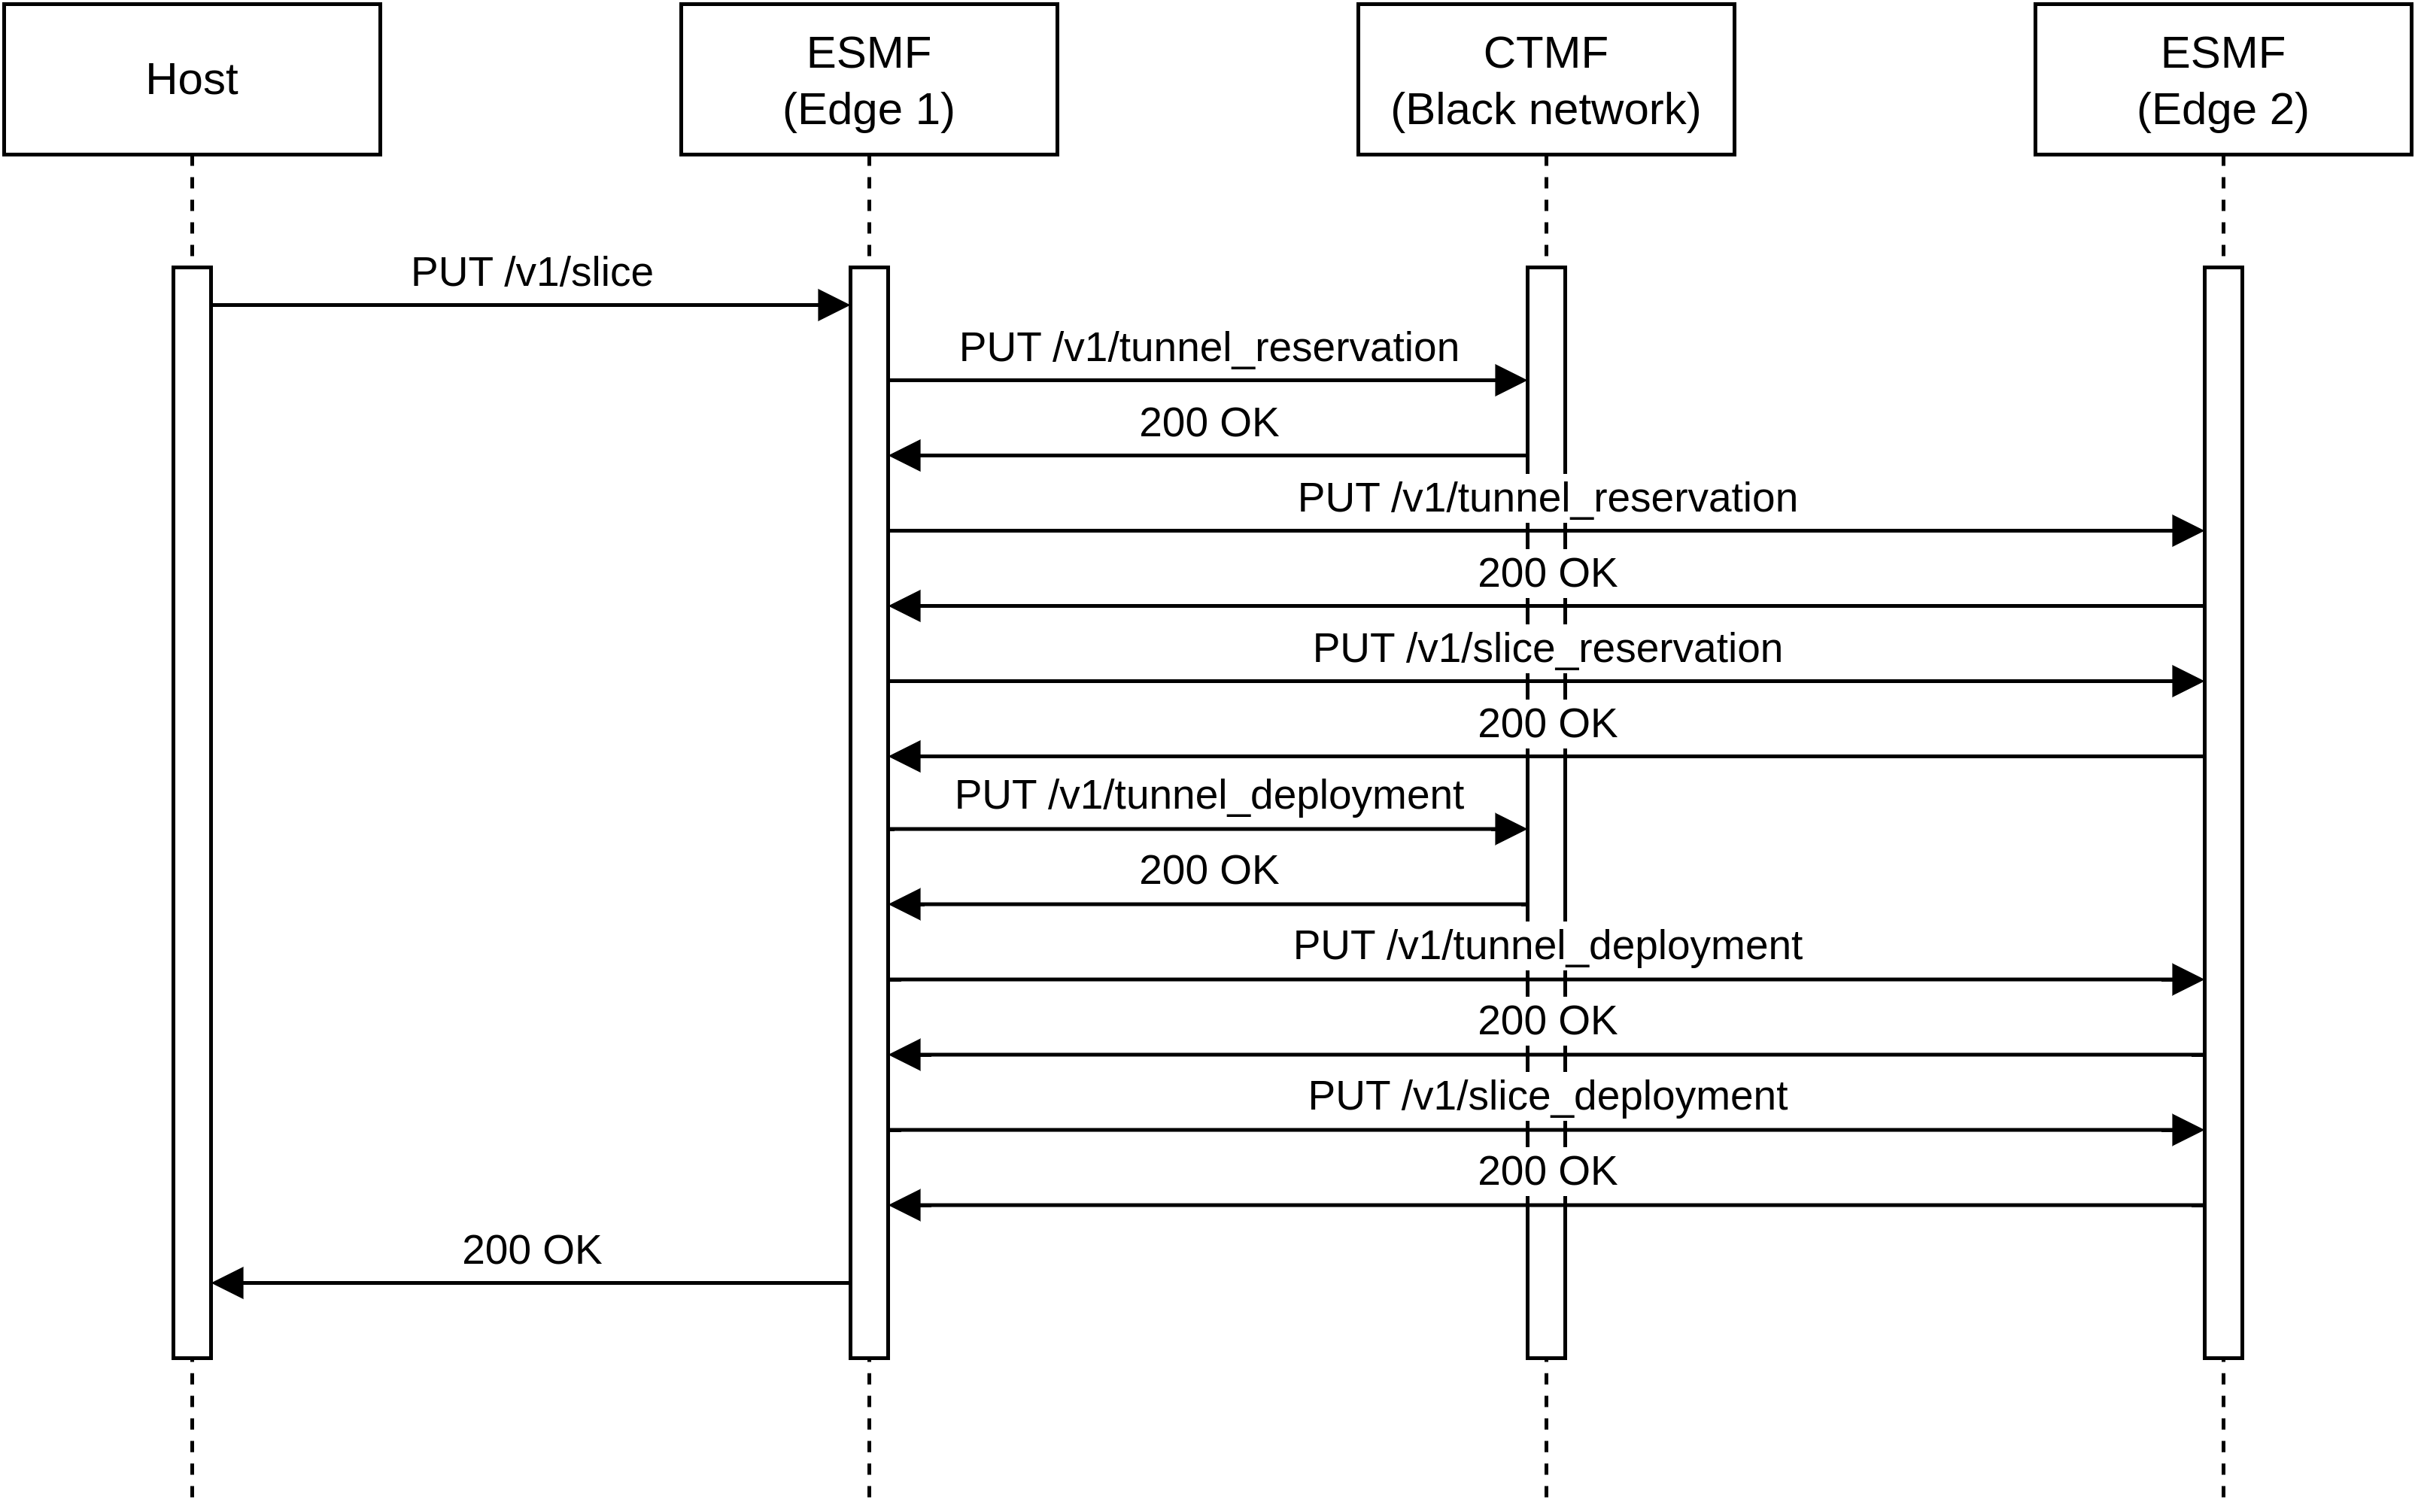
\includegraphics[width=\linewidth]{images/chapter_6/slice_creation_coordination.png}
    \caption[Slice creation on the coordinators]{Successful \acrshort{esmf} and \acrshort{ctmf} synchronization to create a slice illustrated in a sequence diagram. The coordinator \acrshort{esmf} that has been contacted by the host will contact all other domain coordinators to check whether the slice and the tunnel generated by the \acrshort{esmf} is feasible first, before instructing everyone to deploy. Finally the \acrshort{esmf} responds back to the coordinating host to indicate successful slice creation. If any steps fail, everything will be rolled back with removal requests and the host would receive a negative reply. If there is more than one \gls{blacknetwork}, the requests for the \acrshort{ctmf} need to be applied on each of them.}
    \label{fig:slice_creation_synchronization}
\end{figure}
\begin{figure}[H]
    \centering
    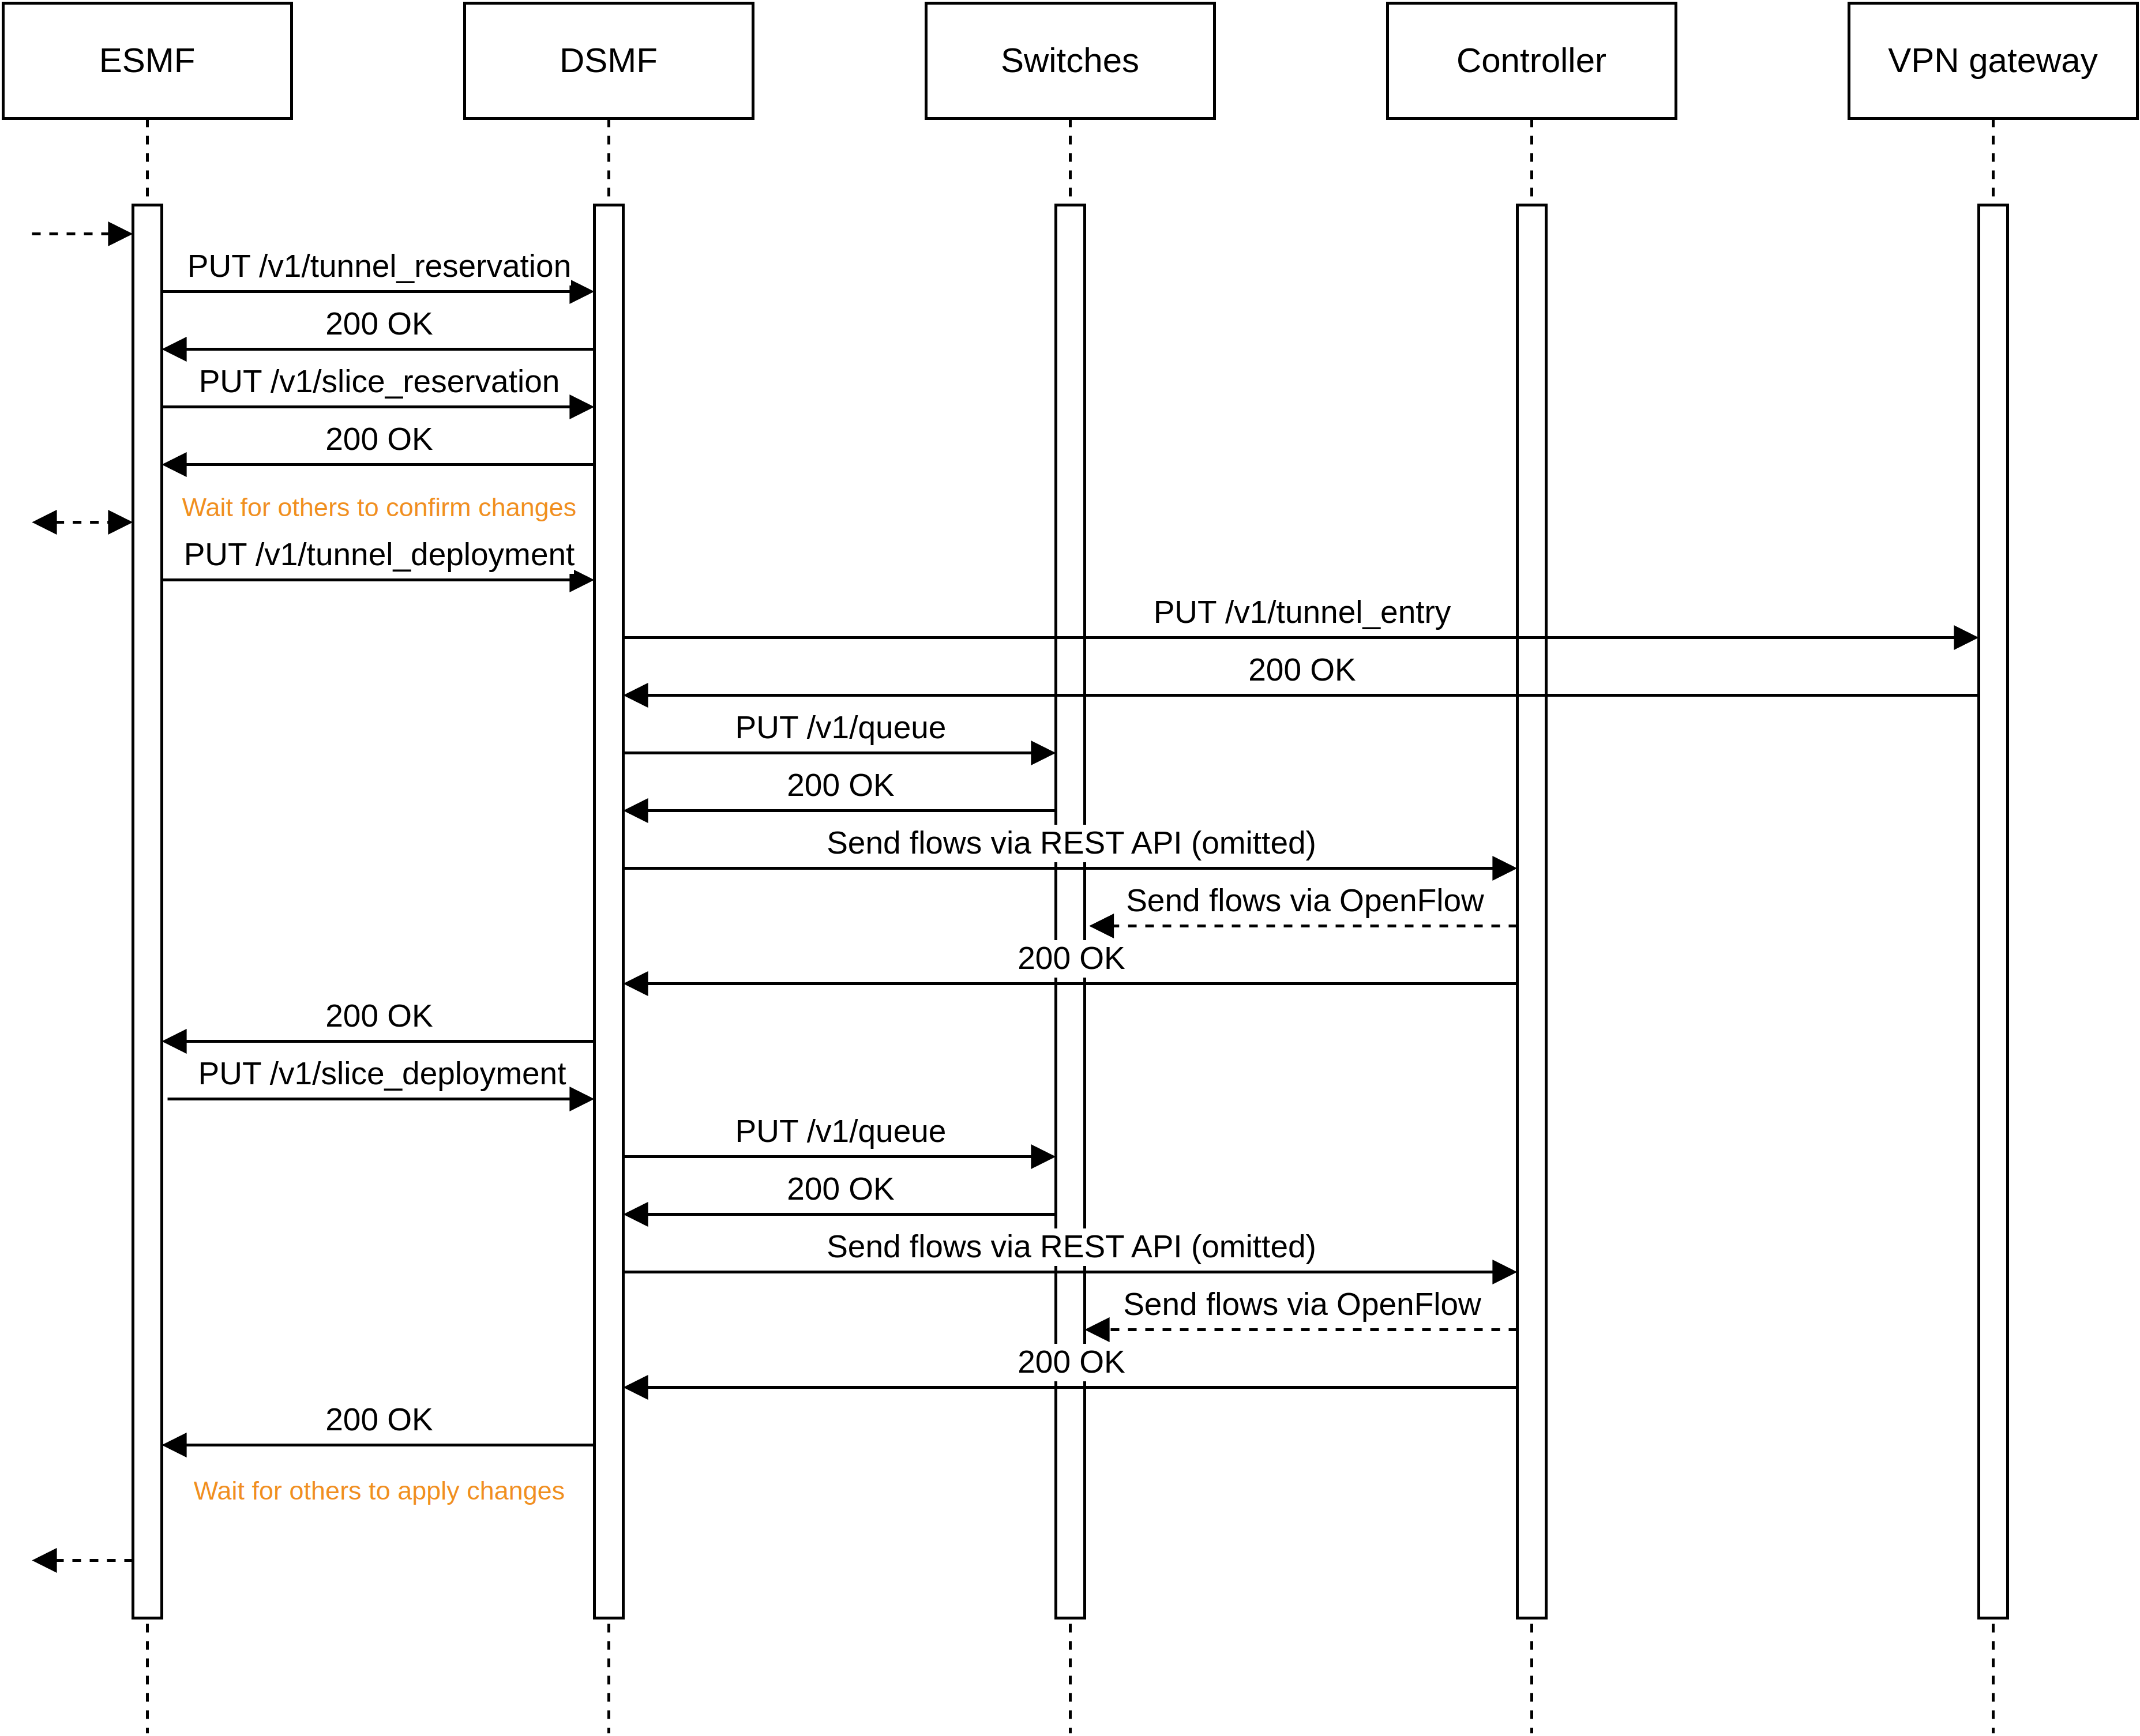
\includegraphics[width=\linewidth]{images/chapter_6/slice_creation_edge.png}
    \caption[Slice creation on an \gls{edgenetwork}]{Communication between \acrshort{esmf}, \acrshort{dsmf}, controller, switches and \acrshort{vpn} gateway on the edge to create a slice illustrated in a sequence diagram. The process seen here deploys the slices and tunnels of a single \gls{edgenetwork}. Requests might be in larger quantity when multiple slices and tunnels get deployed or multiple switches are present. The \acrshort{esmf} will contact the \acrshort{dsmf}, which will then contact the data plane \acrshort{vnf}s to deploy the actual functionality. Everything is guarded by reservations upfront. The dotted arrows to the left indicate synchronization efforts from other \acrshort{esmf}s or communication with the requesting host.}
    \label{fig:slice_creation_edge}
\end{figure}
\begin{figure}[H]
    \centering
    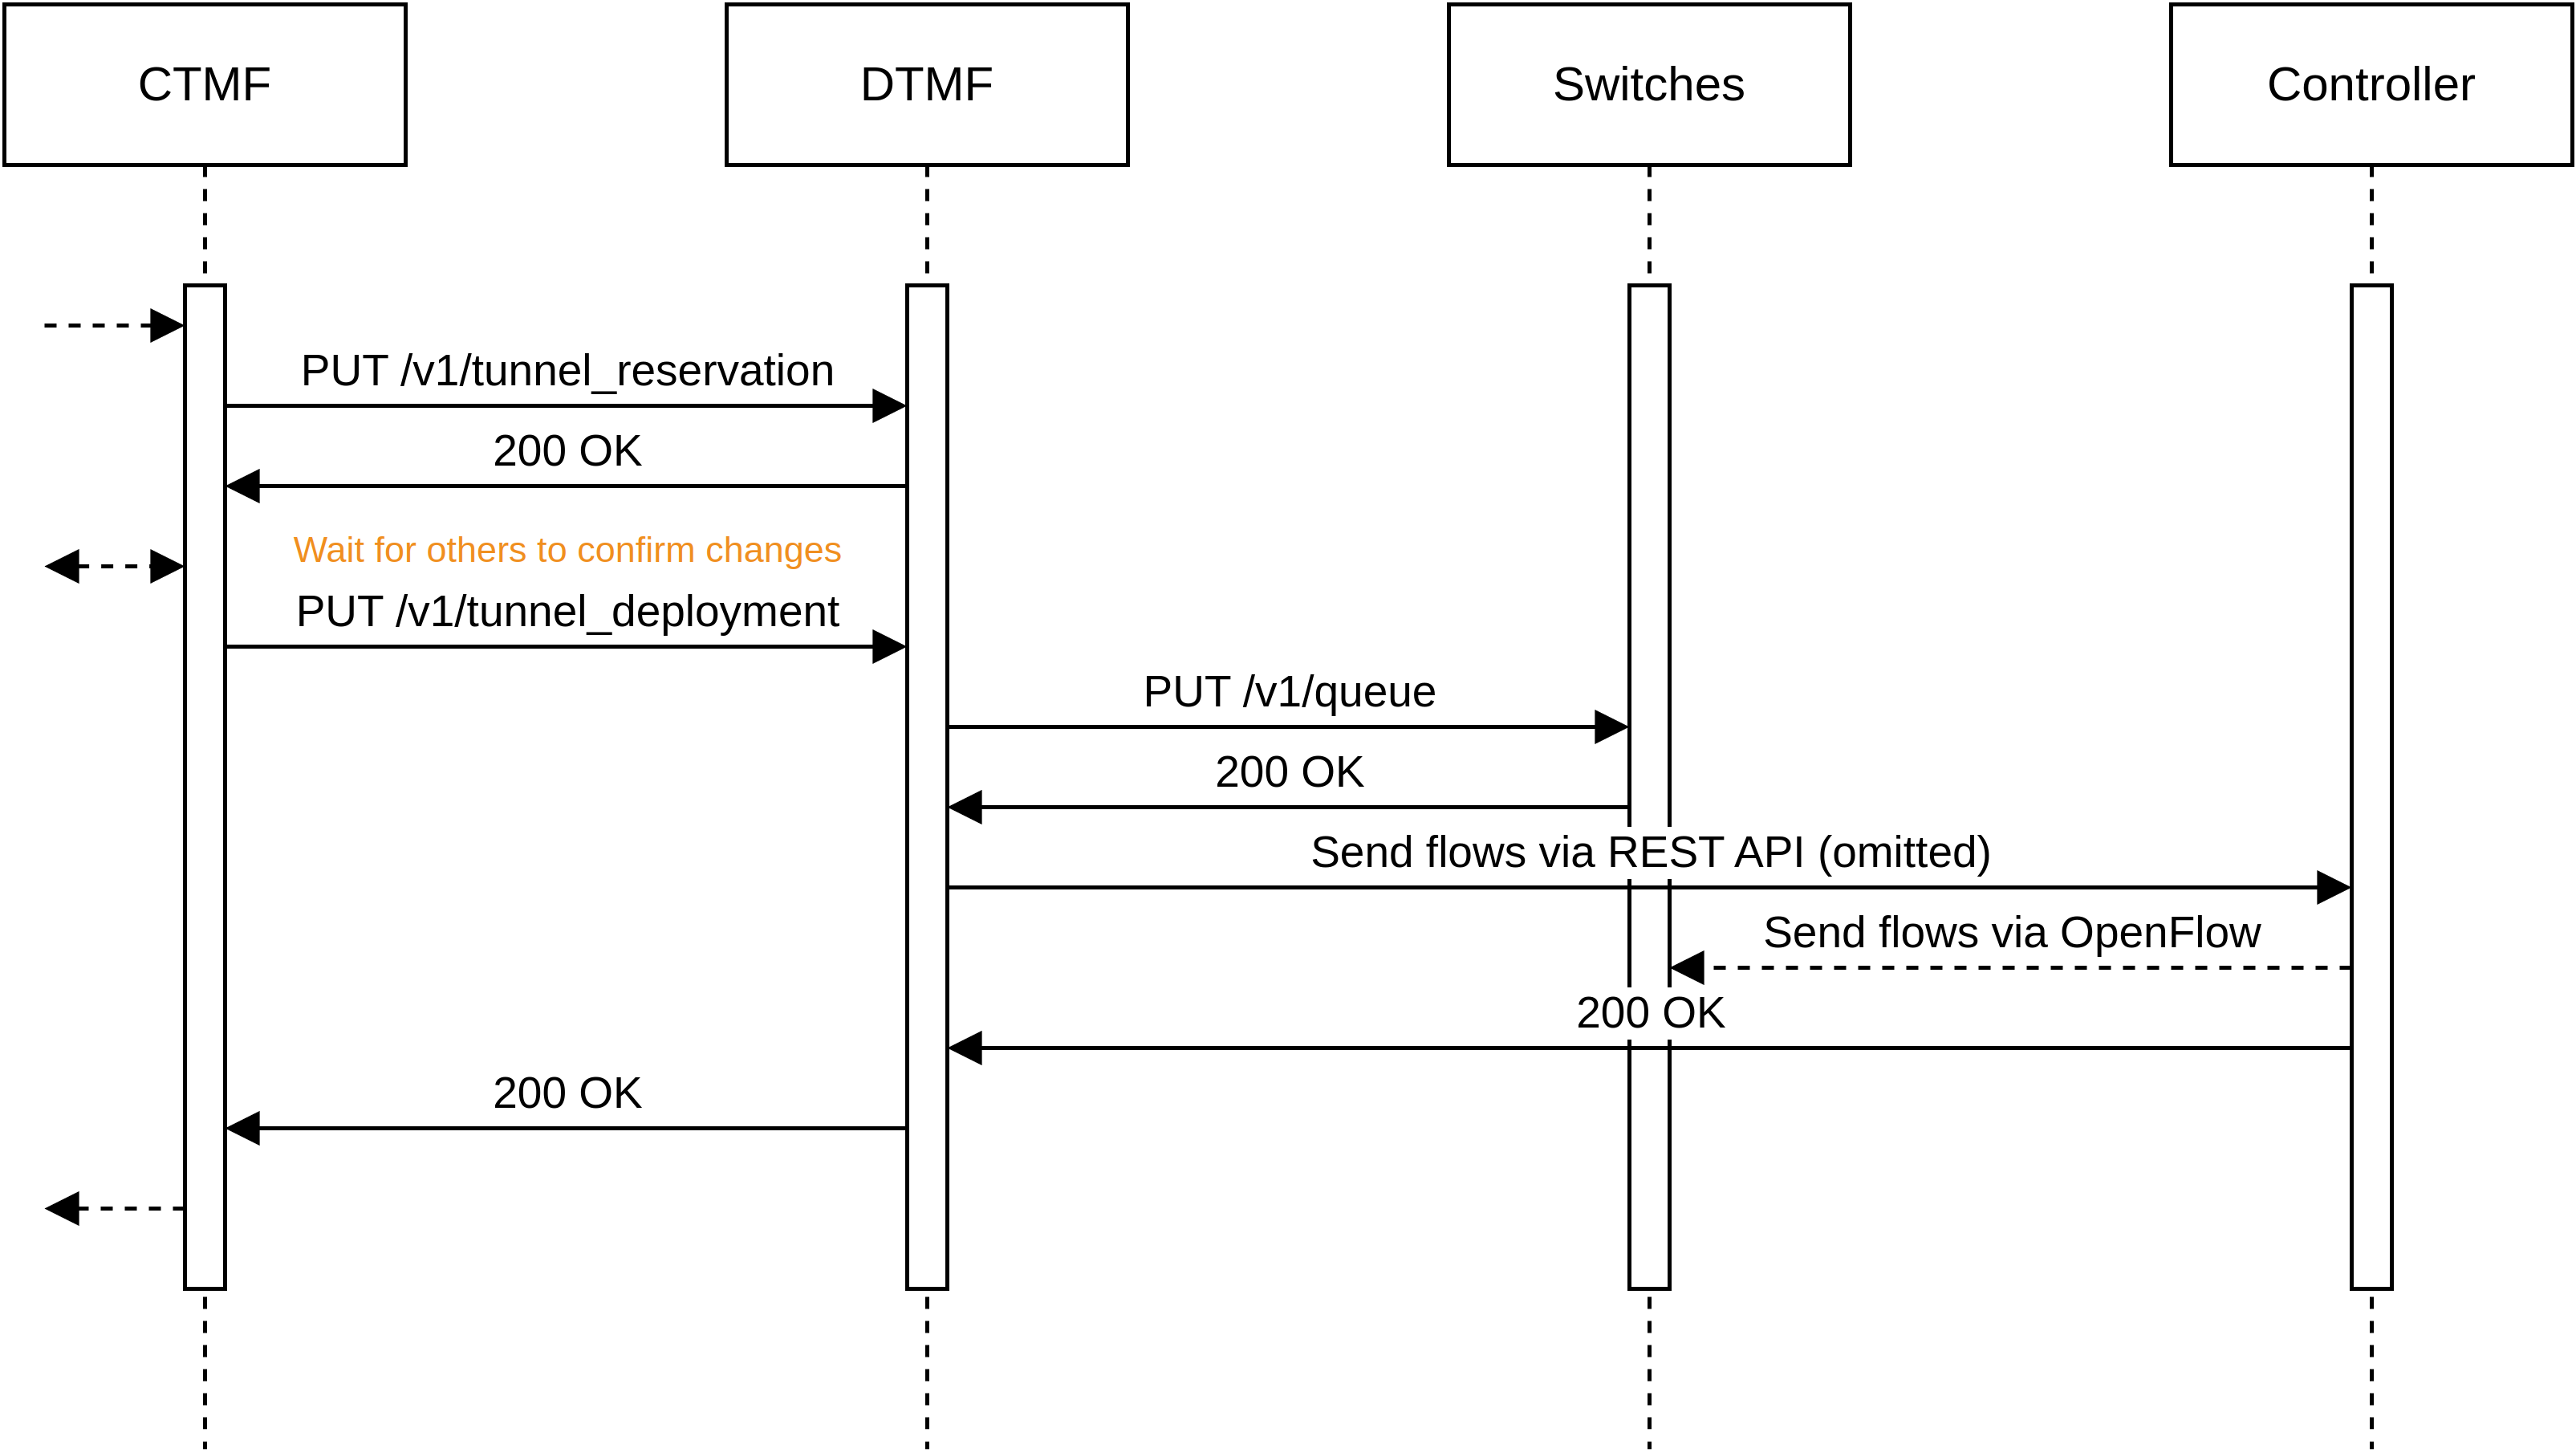
\includegraphics[width=\linewidth]{images/chapter_6/slice_creation_bn.png}
    \caption[Slice creation on a \gls{blacknetwork}]{This figure shows the communication between \acrshort{ctmf}, \acrshort{dtmf}, controller and switches on the \gls{blacknetwork} in a sequence diagram in order to create tunnels. There are no \acrshort{vpn} gateways on \gls{blacknetwork}s, so they do not appear here as compared to the figure on \gls{edgenetwork}s. As previously with \acrshort{esmf} and \acrshort{dsmf}, the \acrshort{ctmf} will contact the \acrshort{dtmf}, which will then instruct the controller and switches to deploy the tunnel functionality. Everything is guarded by reservations upfront. The dotted arrows to the left indicate synchronization efforts from other \acrshort{esmf}s. If there are multiple switches the requests are repeated for each of them.}
    \label{fig:slice_creation_bn}
\end{figure}

\newpage

\subsubsection{Slice removal}
In order to remove a slice the steps mentioned above are basically reversed. In this case we do not use the two-phase commit protocol, as when failing to synchronize the same drawbacks as mentioned above occur, which could be solved by future implementations with ease by removing dangling deployments.

As for the creation of one or multiple slices, the coordinating \acrshort{esmf} is contacted again to remove these slices. The \acrshort{esmf} will create a list of all slices and tunnels affected and issue a removal for them. A tunnel is removed when no slices remain on the tunnel, else the tunnel may be adapted to include less capacity. The \acrshort{esmf} will contact all other participating domain coordinators and state slices and tunnels to be removed. Each domain coordinator, including the coordinating \acrshort{esmf} will then contact the infrastructure coordinator of their domain requesting a removal of all tunnels and slices that are supposed to be removed. The infrastructure providers will then use the before mentioned \acrshort{api}s to remove all components. When everyone reports back a positive result, the host is informed about the positive result of the removal.

As with the previous section, the entire process of removing a slice can also be viewed as sequence diagrams for the state synchronization (see Figure \ref{fig:slice_removal_synchronization}), the communication on the \gls{edgenetwork}s (see Figure \ref{fig:slice_removal_edge}) and on our \gls{blacknetwork}s (see Figure \ref{fig:slice_removal_bn}).

\begin{figure}[H]
    \centering
    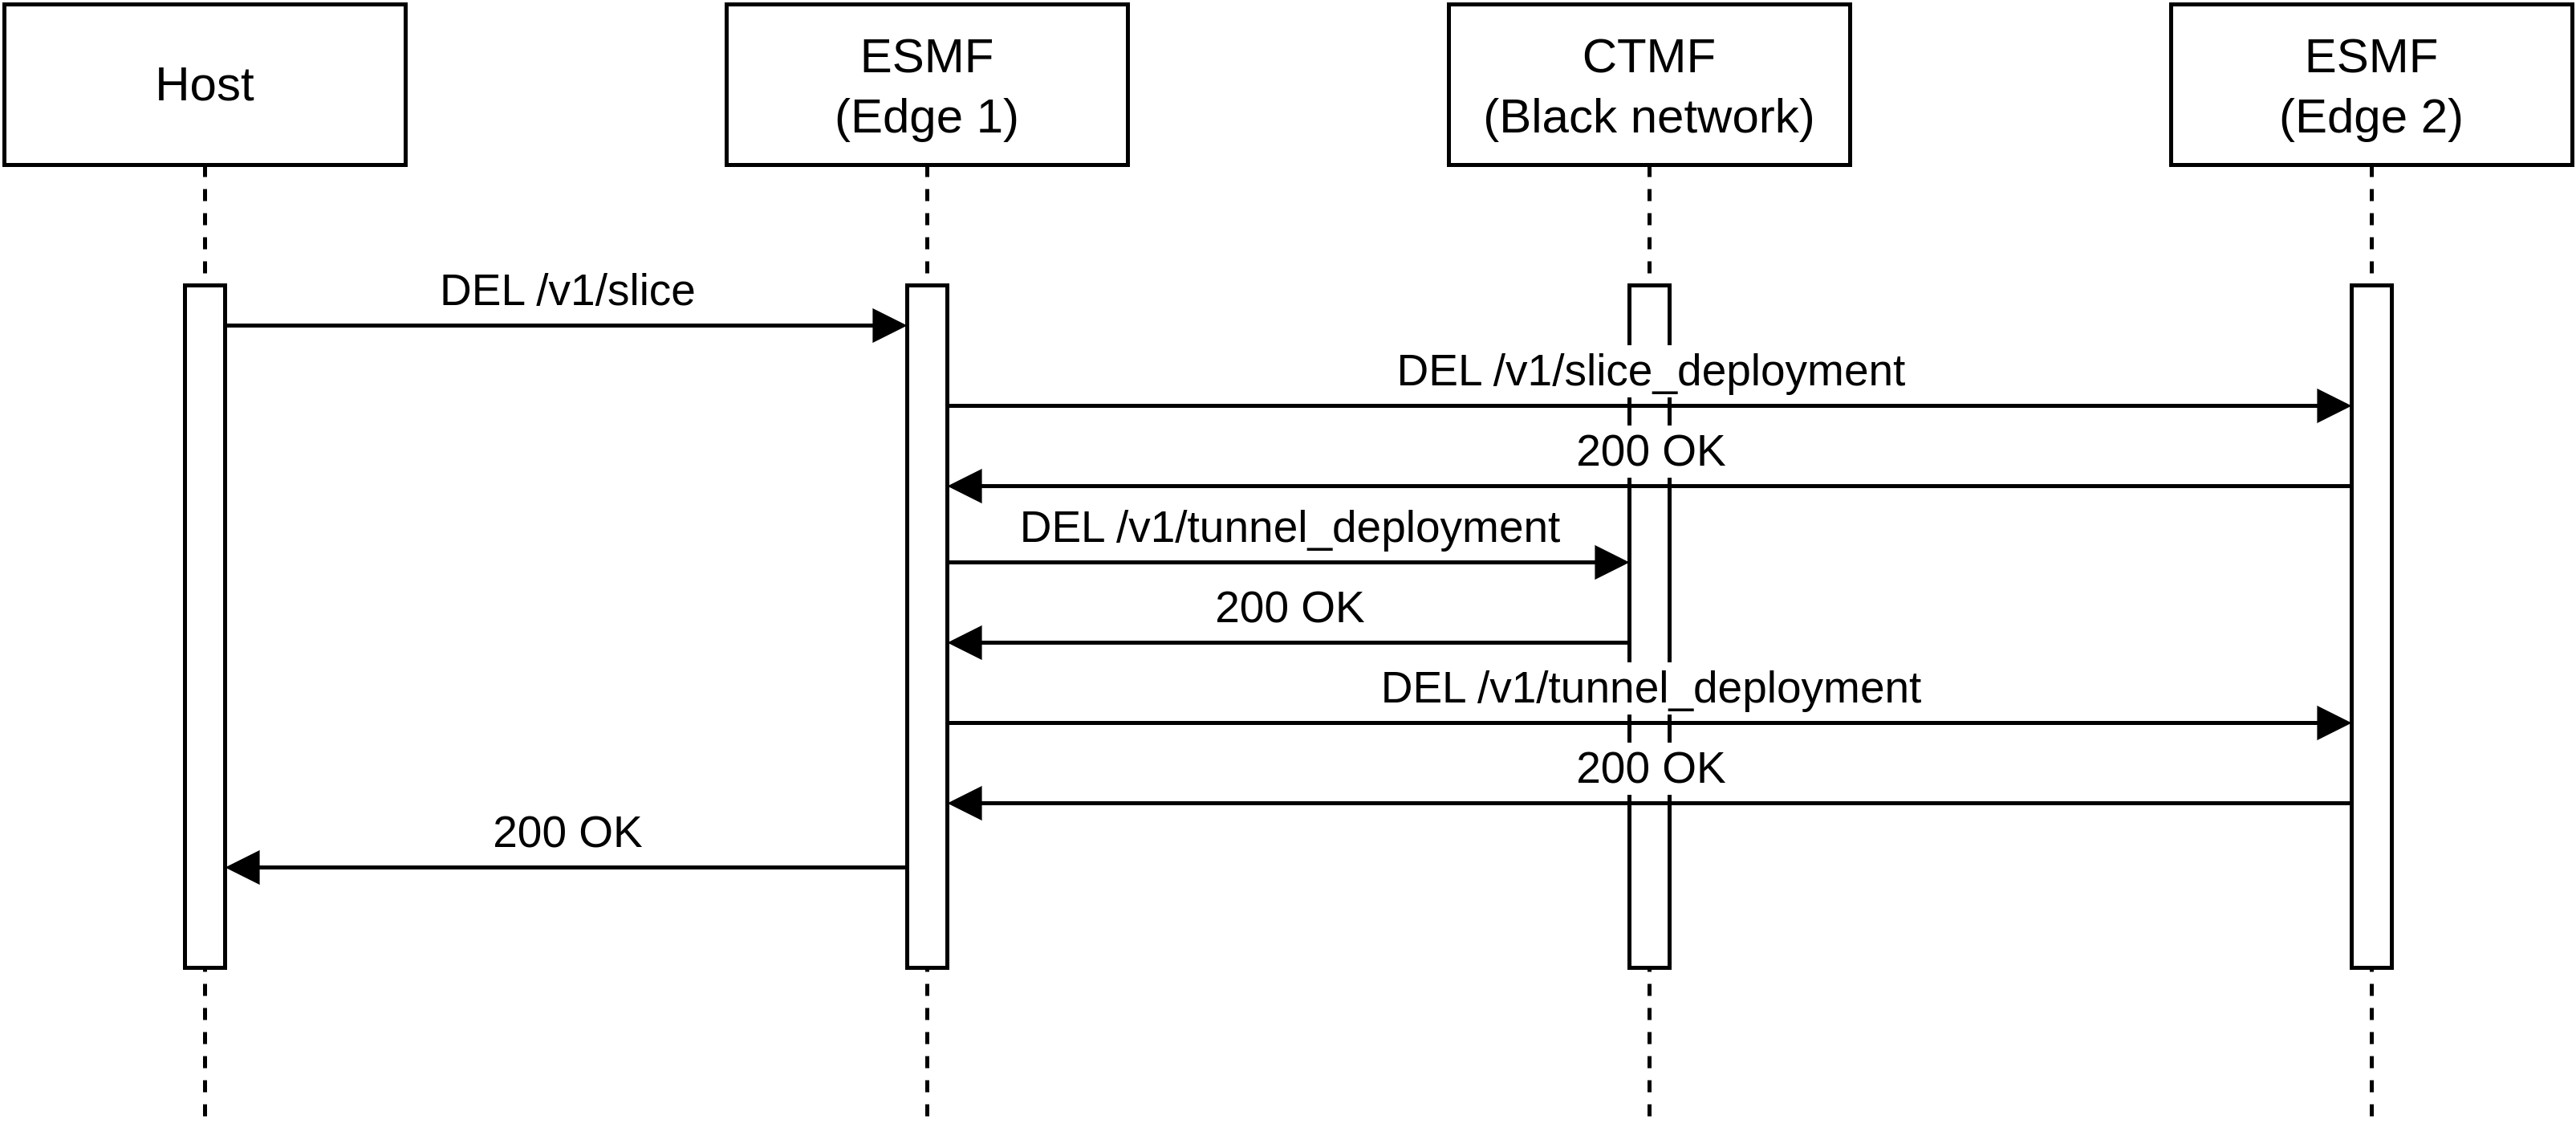
\includegraphics[width=\linewidth]{images/chapter_6/slice_removal_coordination.png}
    \caption[Slice removal on the coordinators]{Removal of slices on the domain coordinator level illustrated in a sequence diagram. The coordinator \acrshort{esmf} that has been contacted by the host will contact all other domain coordinators to remove the slice and all tunnels that have to be removed with the slice or that need to be adapted. Once everyone reports successful removal, the successful result is reported back to the host. If anyone reported a failure to remove, the host will receive a negative reply. If there is more than one \gls{blacknetwork}, the requests for the \acrshort{ctmf} need to be applied on each of them.}
    \label{fig:slice_removal_synchronization}
\end{figure}
\begin{figure}[H]
    \centering
    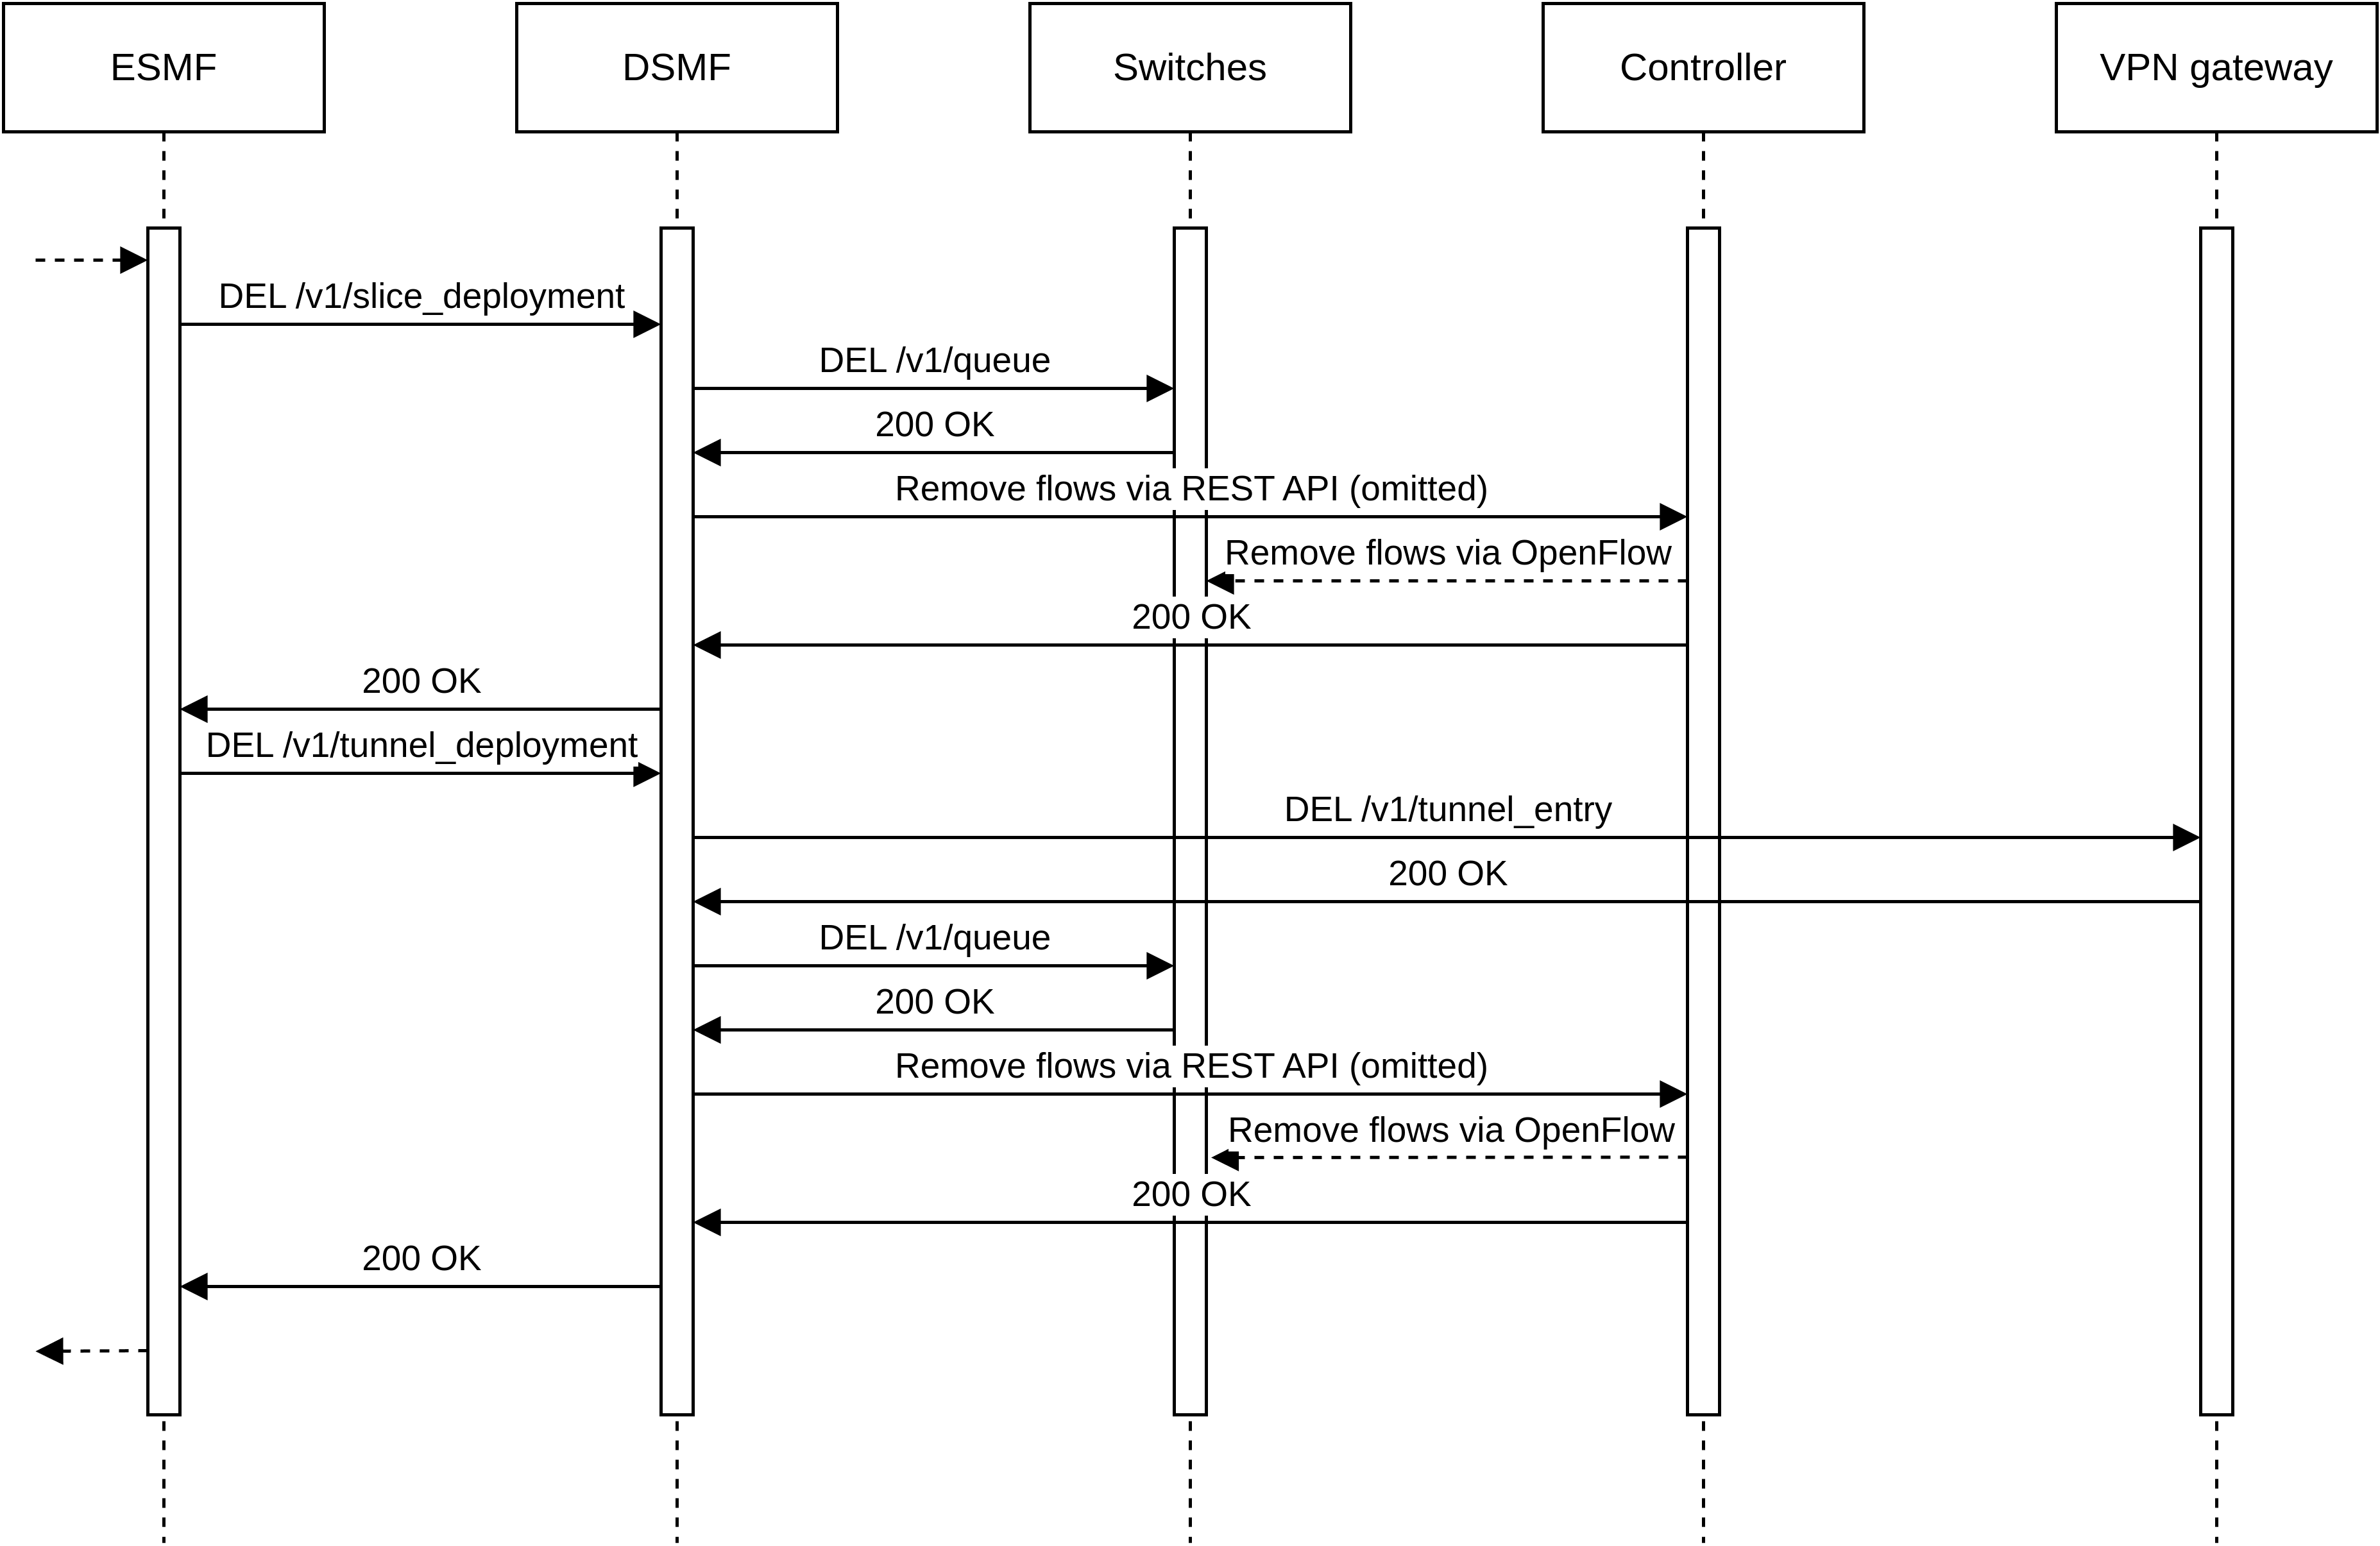
\includegraphics[width=\linewidth]{images/chapter_6/slice_removal_edge.png}
    \caption[Slice removal from an \gls{edgenetwork}]{Sequence diagram showing the removal of slices and tunnels from an \gls{edgenetwork}. The \acrshort{esmf} will contact the \acrshort{dsmf}, which will then instruct controller, switches and \acrshort{vpn} gateway to remove slice and tunnel components. Requests might be in larger quantity when multiple slices and tunnels get removed or multiple switches are present. The dotted arrows to the left indicate synchronization efforts from other \acrshort{esmf}s or communication with the requesting host.}
    \label{fig:slice_removal_edge}
\end{figure}
\begin{figure}[H]
    \centering
    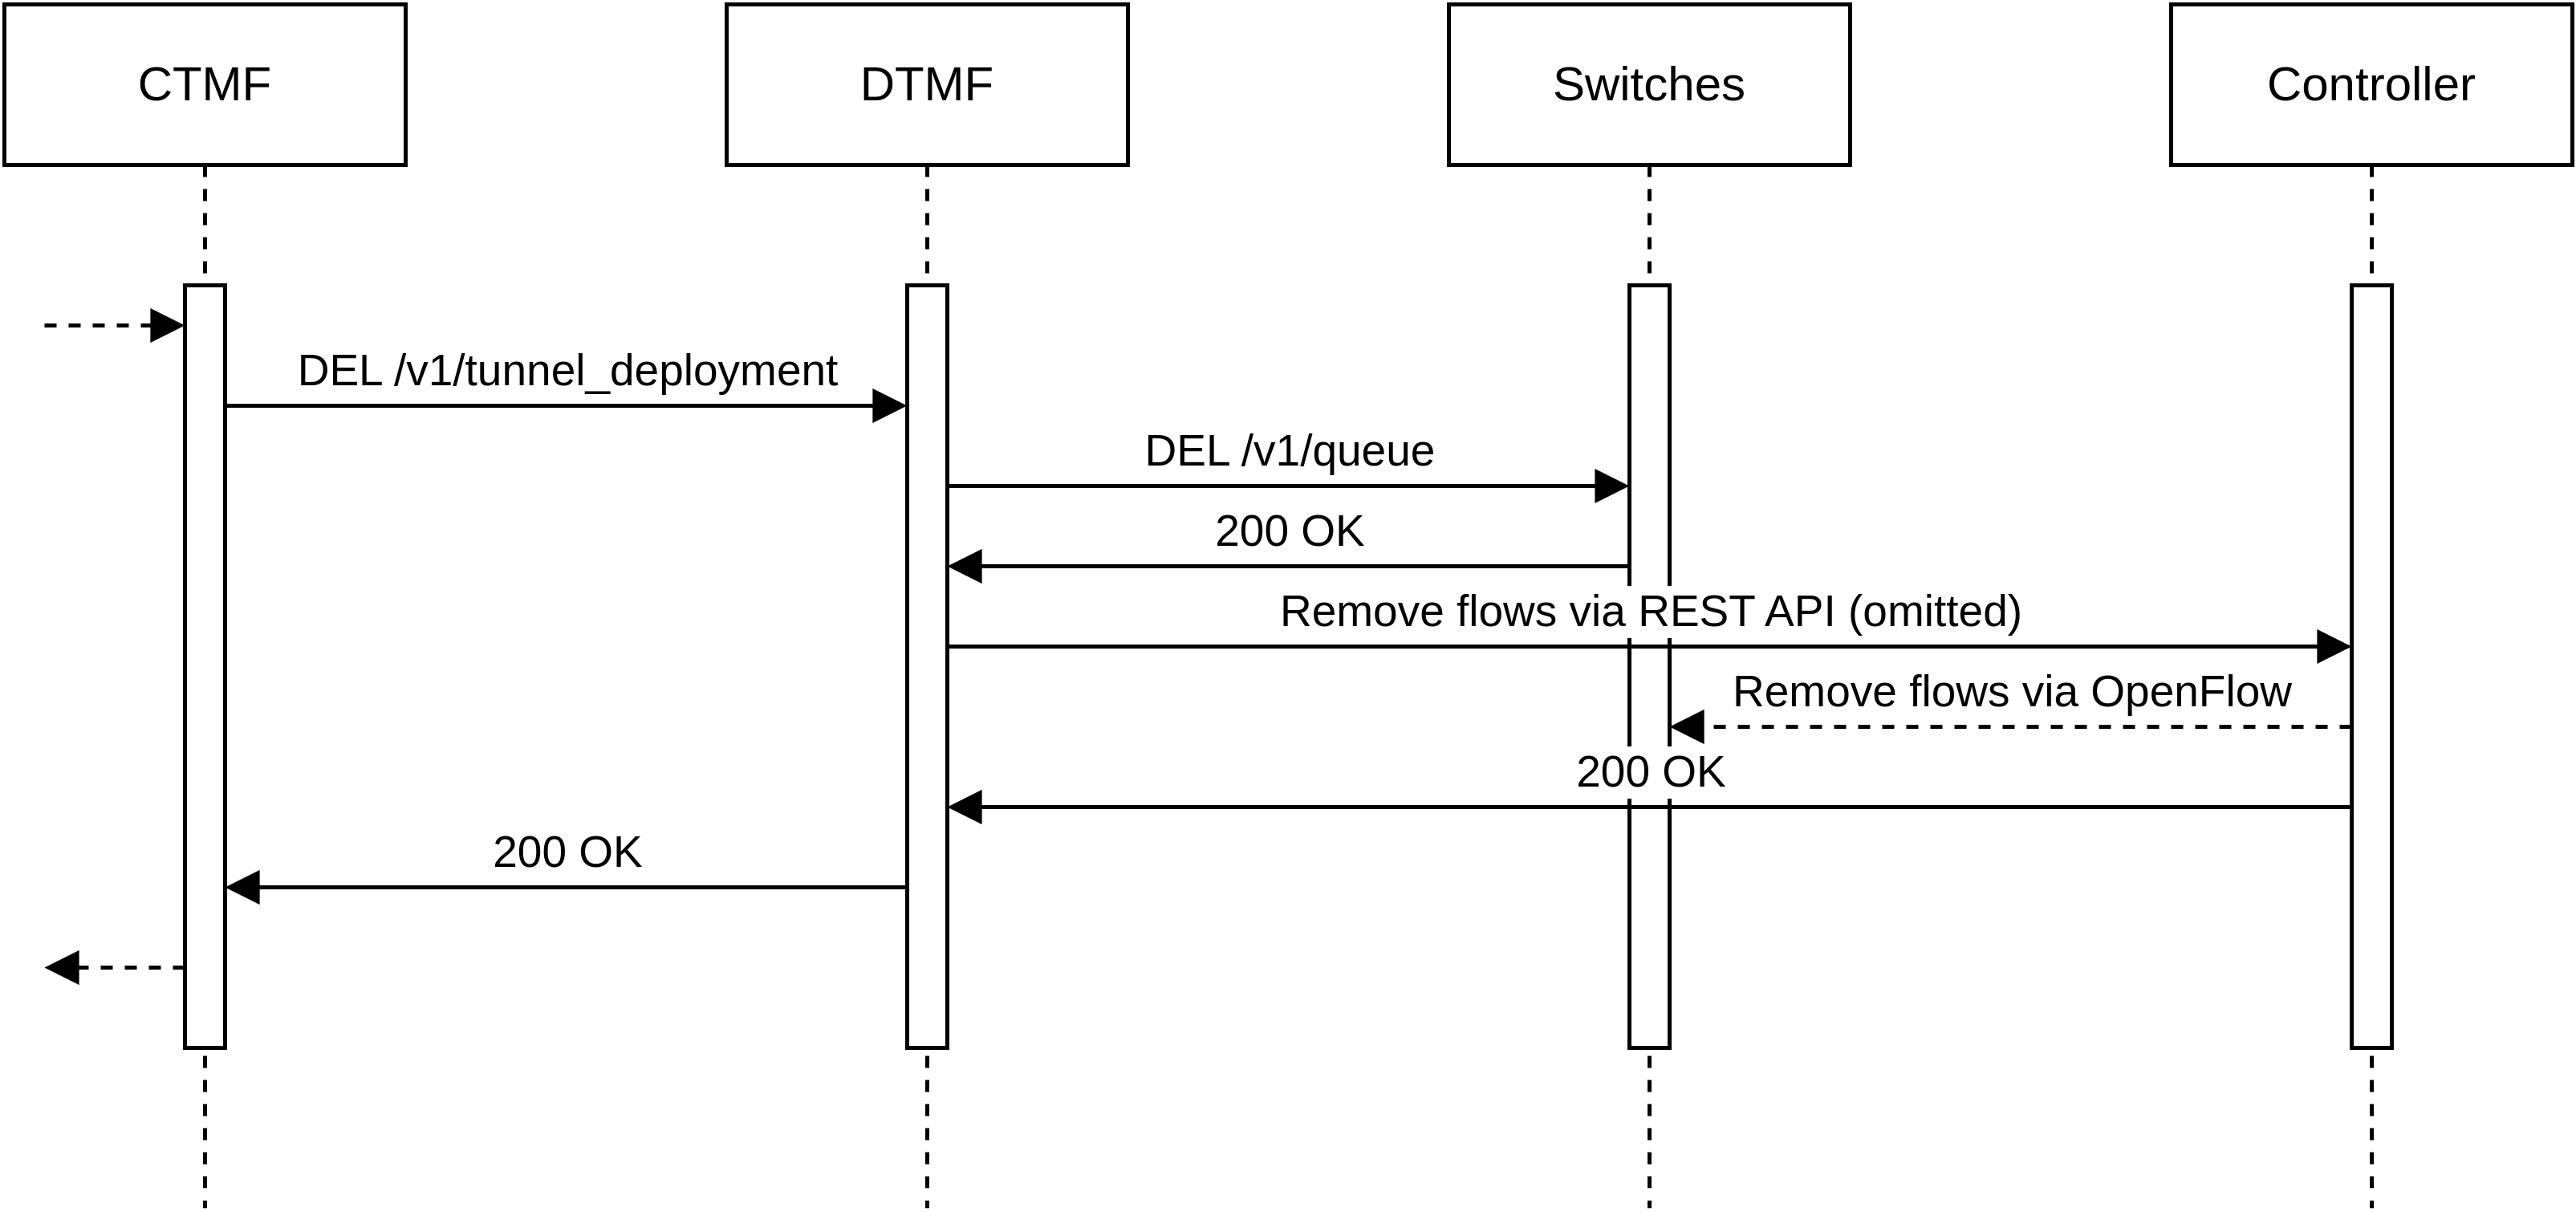
\includegraphics[width=\linewidth]{images/chapter_6/slice_removal_bn.png}
    \caption[Slice removal from a \gls{blacknetwork}]{Sequence diagram showing the removal of tunnels from a \gls{blacknetwork}. The \acrshort{ctmf} will contact the \acrshort{dtmf}, which will then instruct controller and switches to remove the tunnel components. The dotted arrows to the left indicate synchronization efforts from other \acrshort{esmf}s. If there are multiple switches the requests are repeated for each of them.}
    \label{fig:slice_removal_bn}
\end{figure}

\newpage


\section{Components}
In general, all of our \acrshort{vnf}s have been implemented using python. Any version higher than 3.8 should be compatible. The components are shipped as python packages and are pre-installed into \acrshort{lxc} containers (small footprint containers running on the linux platform) \cite{lxc} for use in our validation later. All images come with preinstalled common software and utilities to be able to carry out our validation later and to realize our attackers. Currently included are \textit{iputils-ping} \cite{iputils}, \textit{net-tools} \cite{net-tools}, \textit{iperf3} \cite{iperf3}, \textit{\gls{wireguard}} \cite{wireguard}, \textit{tcpdump} \cite{tcpdump}, \textit{ifstat} (part of \textit{iproute2} \cite{iproute2}), \textit{hping3} \cite{hping3} and \textit{sockperf} \cite{sockperf}. If a package is missing on certain components, it can be integrated by adapting the setup instructions if required.

Some images have additional software apart from above. These and their functionality are stated here:

\paragraph{Application plane components} All components on the application plane (\acrshort{esmf}, \acrshort{ctmf}, \acrshort{dsmf}, \acrshort{dtmf}) have their designated server implementation running, performing their coordination and management duties described in Section \ref{impl_specification}.

\paragraph{Switches} The switches currently use \Gls{ovs} (OVS) \cite{openvswitch} to deploy \acrshort{sdn} switch functionality. Additionally a switch server implementation is executed which issues commands to manage queues and ingress policies on switch ports.

\paragraph{Controller} The controller is realized by utilizing the \Gls{ryu} \cite{ryu} with the common RYU \acrshort{rest} \acrshort{api} \cite{ryu-rest}.

\paragraph{\acrshort{vpn} gateways} The \acrshort{vpn} gateways run a server implementation that allows the creation of \gls{wireguard} \cite{wireguard} tunnel entries. The details of these tunnel entries are explained below in Section \ref{impl_concepts}.


\section{Concepts and configuration}
\label{impl_concepts}
Now that we have established how we wish to deploy tunnels and slices, we still need to specify how the exact configuration on the hardware should be performed.

For simplicity of our implementation, we do not deploy bi-directional slices or tunnels, but rather deploy two uni-directional slices or tunnels to build one single bi-directional one.

A summary of all the flow rules can be seen in figures \ref{fig:routing_source}, \ref{fig:routing_destination} and \ref{fig:routing_bn}.

\subsection{General switch configuration}
To configure a switch we first specify ingress limits on all interfaces, setting the maximum allowed rate and burst to 1Gbit/s. This can of course be adapted for other use cases in the future. This is realised by OVS using a token bucket filter. This way the maximum needed computational capacity of our switch can be evaluated better and an upper limit is provided.

\subsection{Slice configuration}
Slices are configured by deploying flows to our slice switches. For this, we install queues to be used by our flows on each switch participating in the slice first that will then be used by our slice flows. To begin creating the flows the switches are first assigned roles.

We first configure the switches between the origin of our slice and the \acrshort{vpn} gateway. We currently always expect that the slice uses a tunnel and therefore has a \acrshort{vpn} gateway it needs to enter.

If there is only one switch, the switch takes the \textit{SRC\_ALL} role, because it contains all functionality of the source network. If there are multiple switches, the first switch will take the \textit{SRC\_ENTRY} role and the last switch the \textit{SRC\_EXIT} role. All switches between will be assigned a \textit{SRC\_TP} role, indicating that they are transport switches on the source network.

\begin{figure}[ht]
    \centering
    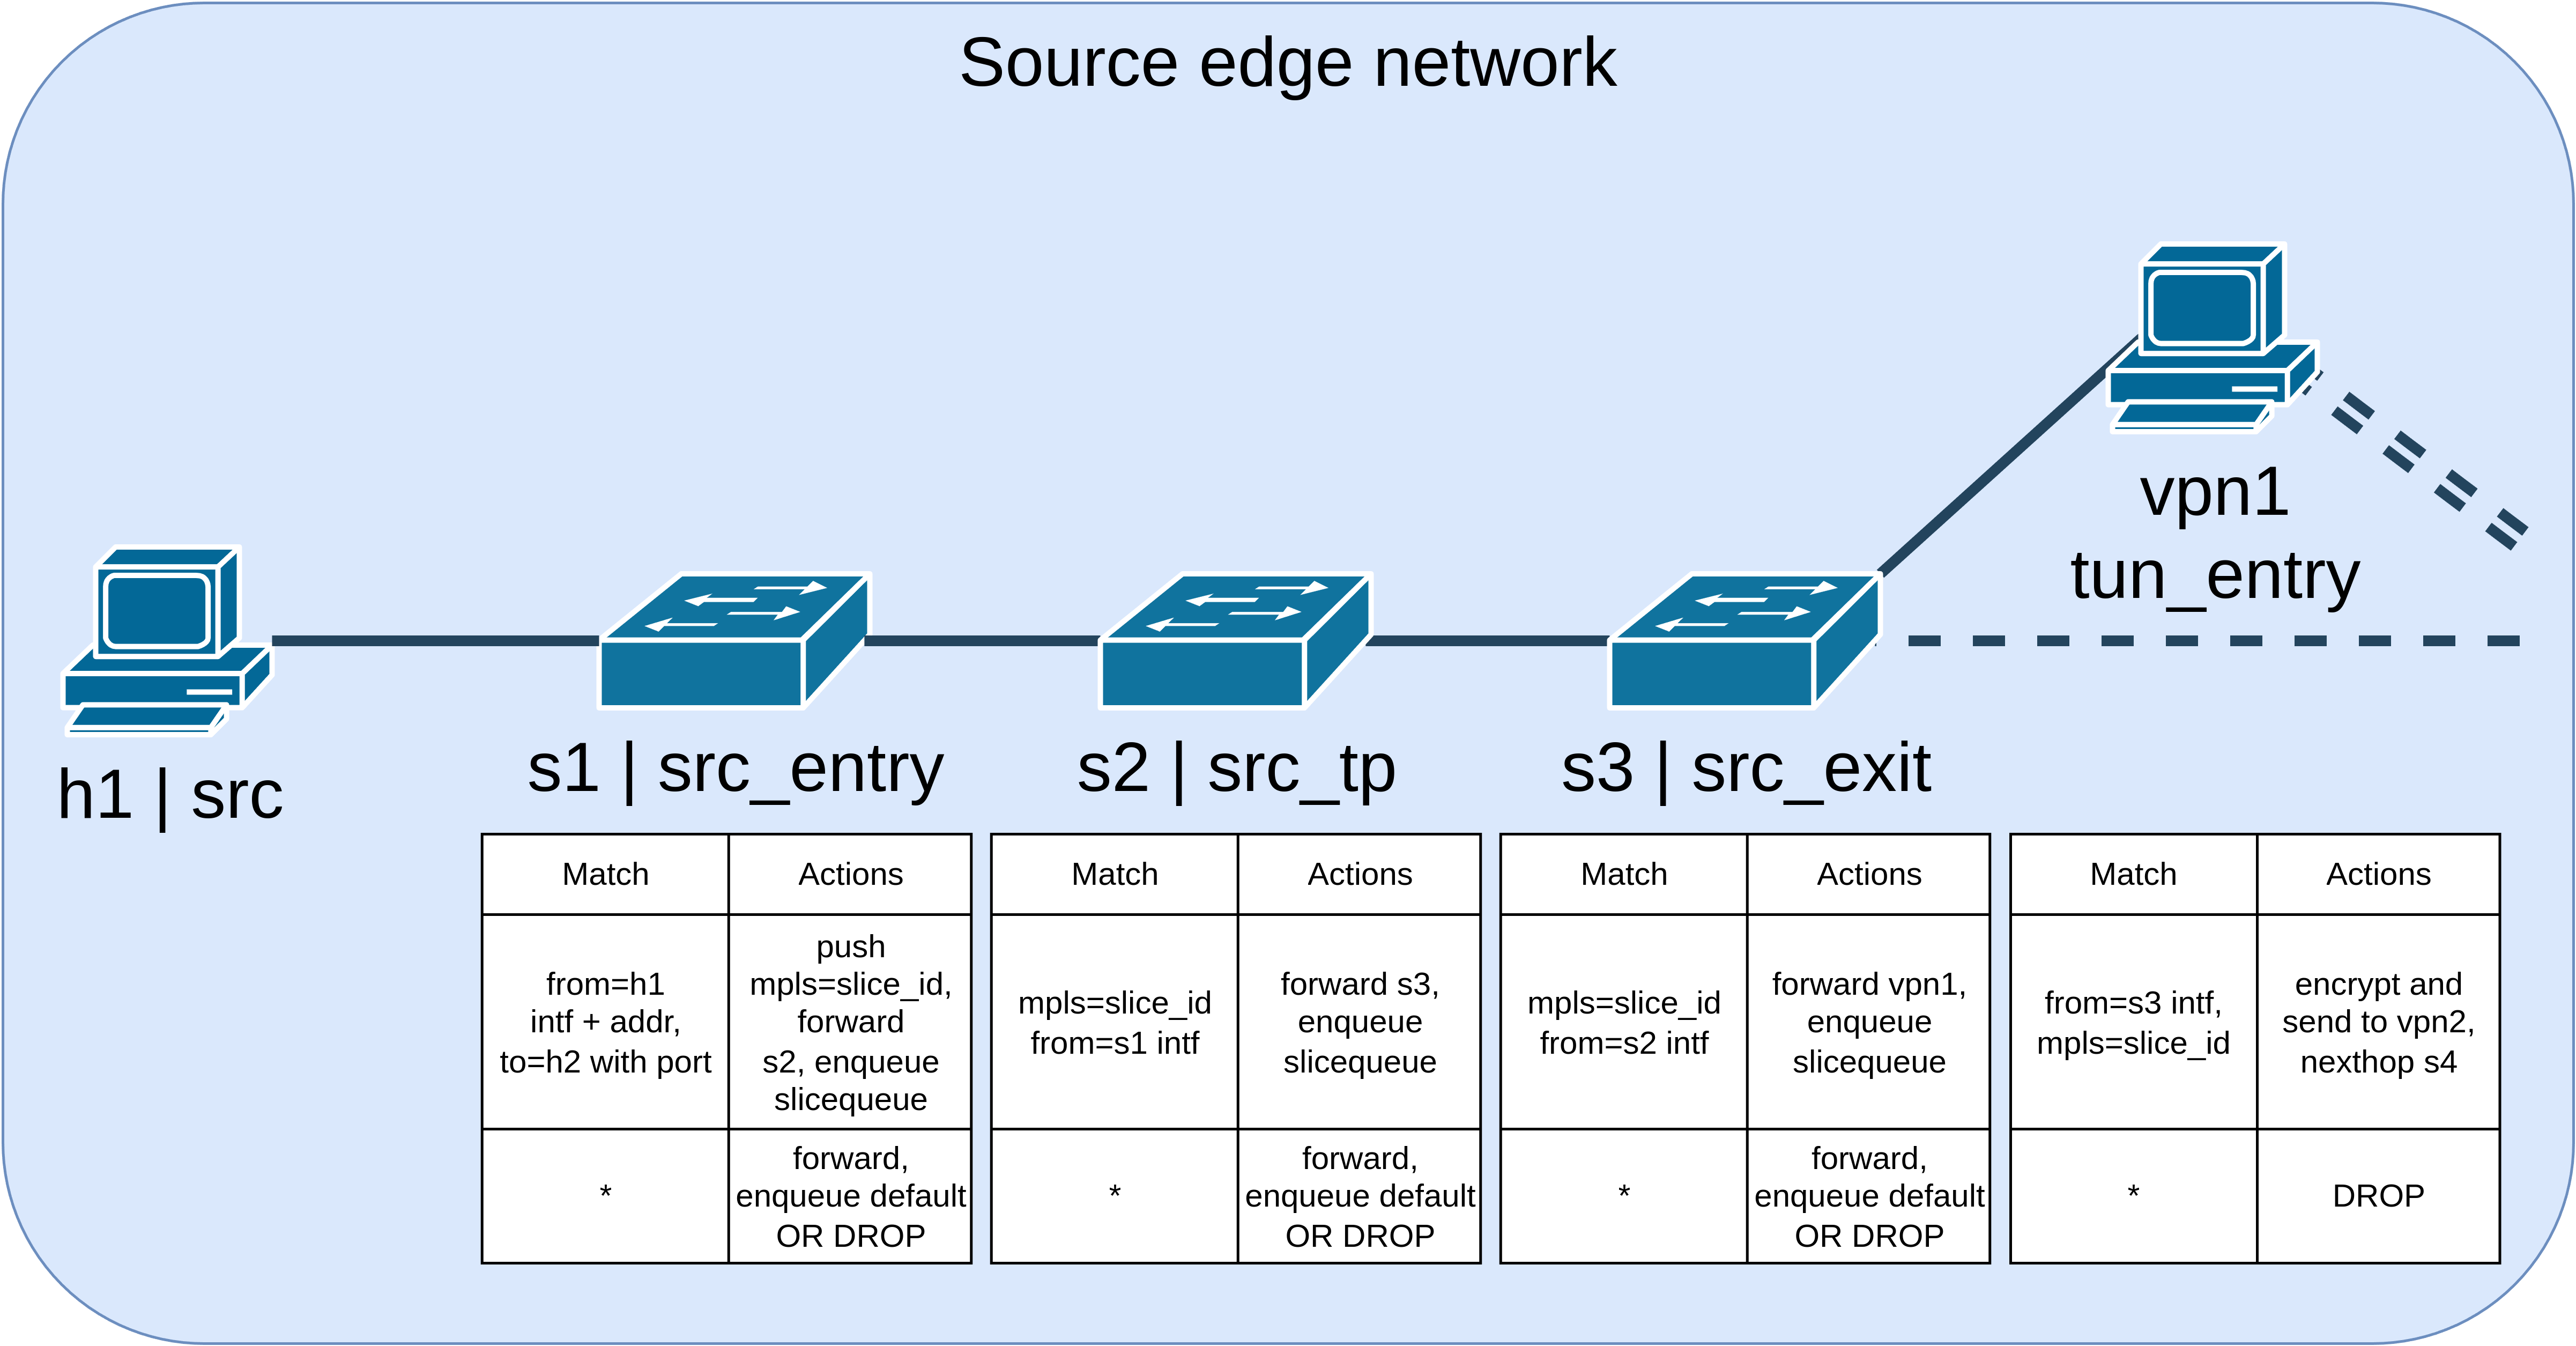
\includegraphics[width=10cm]{images/chapter_6/routing_source.png}
    \caption[Routing on the source \gls{edgenetwork}]{The routing rules on the source \gls{edgenetwork} for the switches and \acrshort{vpn} gateways according to their roles. The dotted lines lead to the first \gls{blacknetwork} switch.}
    \label{fig:routing_source}
\end{figure}

Depending on the role we then deploy the following rules (see Figure \ref{fig:routing_source}):

\paragraph{SRC\_ALL and SRC\_ENTRY} Will verify that a packet matches a slice including the transport destination and port, as well as the incoming interface for authentication purposes. The switch will then tag the packet with an \acrshort{mpls} label using the slice ID as value. The packet will then be forwarded to the next hop.

\paragraph{SRC\_TP and SRC\_EXIT} Will verify that a packet matches a slice by inspecting the slice ID \acrshort{mpls} label and the inbound interface. Will then forward the packet to the next hop. This way, when the next hop is a \acrshort{vpn} gateway, the \acrshort{vpn} gateway will send the slice ID through the tunnel as well.

\paragraph{} Similar to the source network, on the destination network the route from the \acrshort{vpn} gateway to the destination host will be determined and the switches will be assigned roles. These switches will receive the same roles as on the source network, but will be prefixed with \textit{DST} instead. We thus have \textit{DST\_ENTRY} for the switch after the \acrshort{vpn} gateway, then possibly multiple \textit{DST\_TP} switches, before reaching the \textit{DST\_EXIT} switch. As previously, these roles can be combined to form a \textit{DST\_ALL} switch.

\begin{figure}[ht]
    \centering
    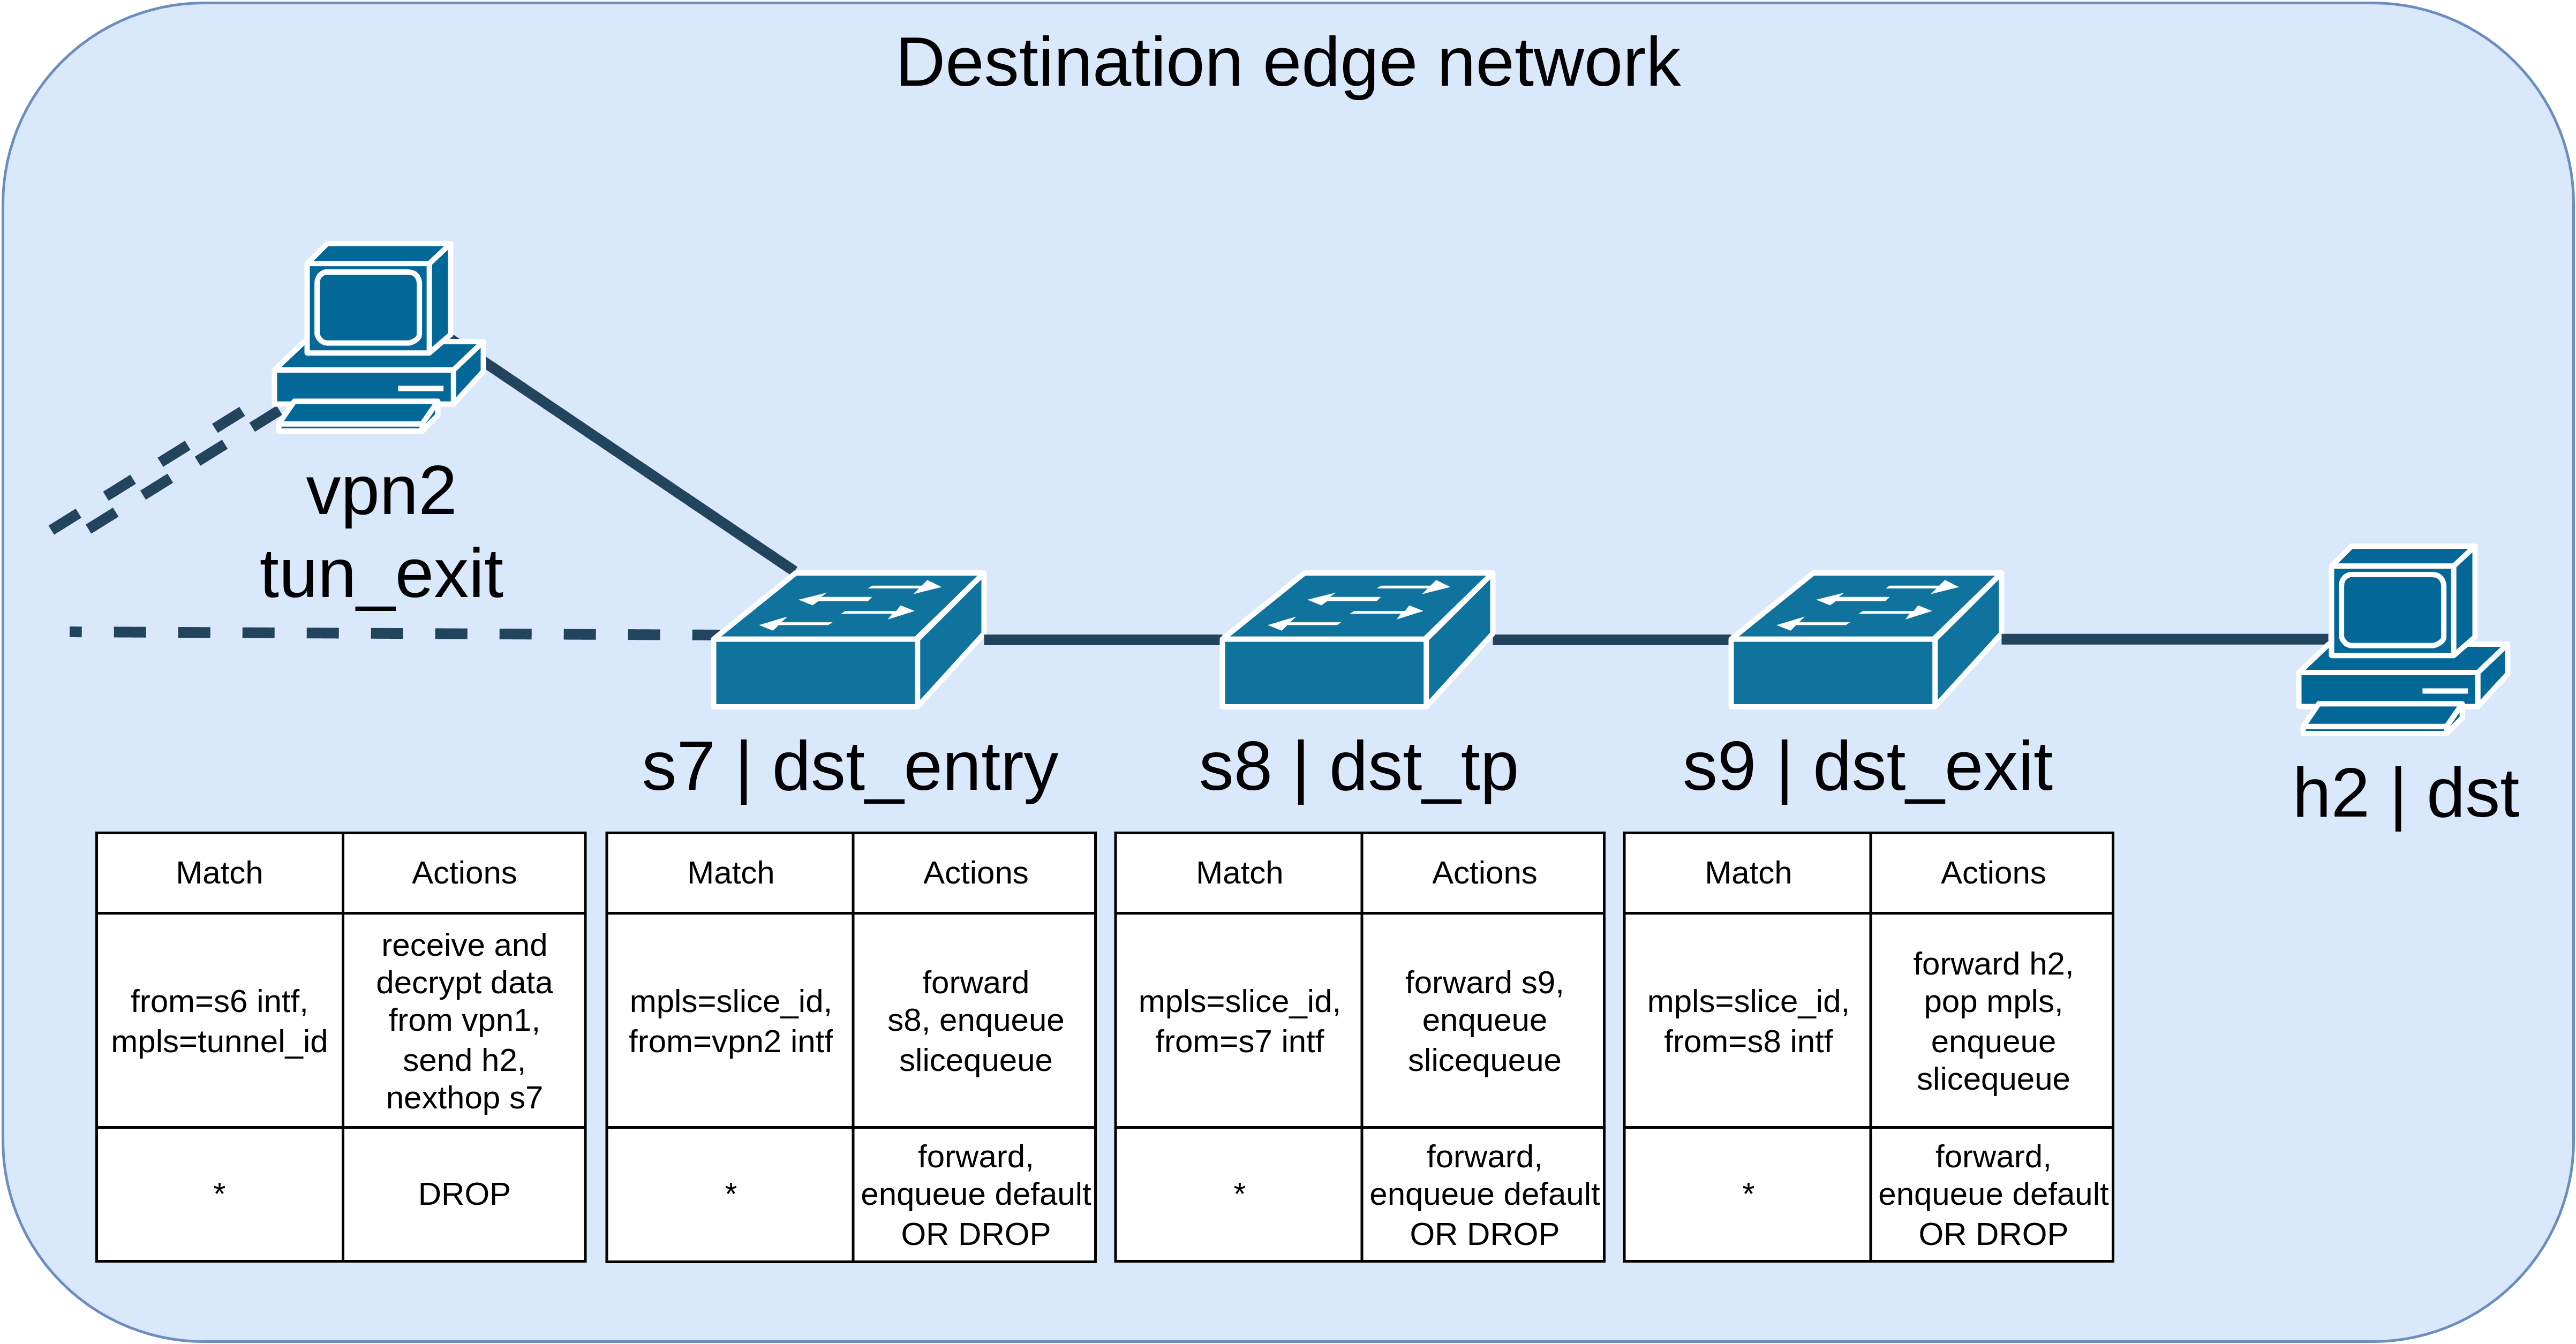
\includegraphics[width=10cm]{images/chapter_6/routing_destination.png}
    \caption[Routing on the destination \gls{edgenetwork}]{The routing rules on the destination \gls{edgenetwork} for the switches and \acrshort{vpn} gateways according to their roles. The dotted lines lead to the last \gls{blacknetwork} switch.}
    \label{fig:routing_destination}
\end{figure}

Depending on the role we then deploy the following rules (see Figure \ref{fig:routing_destination}):

\paragraph{DST\_ENTRY and DST\_TP} Will verify that a packet matches a slice by checking the slice ID \acrshort{mpls} label and the inbound interface. Will then forward the packet to the next hop.

\paragraph{DST\_ALL and DST\_EXIT} Will verify that a packet matches a slice by checking the slice ID \acrshort{mpls} label and the inbound interface. Will then remove the slice ID \acrshort{mpls} label and forward the packet to the next hop. This way the destination host will receive the original packet without any \acrshort{mpls} labels or other additional headers attached to it.

\paragraph{} All switches may also forward traffic on a default slice, where all other traffic resides. This is however not subject to our coordination and thus also not part of our implementation. The default slices will be manually configured in our validation experiments later with adequate resource limitations to not impede on our isolated slices. This feature could be added to the implementation in the future to dynamically resize the default slice and to not under-provision the traffic allocation to all other devices. Without any additional configuration currently all other traffic is blocked.

\paragraph{} As one can see, there are multiple switch roles per network that employ the same rules. This has been implemented this way to provide flexibility for future adaptations, so that potentially different routing rules can be realized in the future, where these roles would not behave identically. However there always has to be at least one switch on the source network and on the destination network before and after the \acrshort{vpn} gateway respectively.

\subsection{Tunnel configuration}
\label{impl_tunnel_config}
Concerning our tunnels we will use a similar strategy to the slices themselves, but need to allocate a tunnel entry and a tunnel exit first.

\paragraph{Tunnel entry} The tunnel entry will be created on the corresponding \acrshort{vpn} gateway on the source network. The tunnel entry will be a \gls{wireguard} tunnel that is configured in pair with the remote \gls{wireguard} tunnel entry. The tunnel entry is bound on a port that can be identified by the \gls{blacknetwork} switches later and that is assigned to the tunnel.

Because \gls{wireguard} is a layer 3 tunnel we will need to create an additional layer 2 tunnel that is established over our \gls{wireguard} tunnel to be able to forward ethernet frames through the tunnel. This has been performed by establishing a \acrshort{gre}TAP tunnel.

Now that we have our tunnel, we still need to route packets to this tunnel. This is achieved by matching packets to slices in a linux qdisc, before redirecting them to their tunnel. If no slices match, the packet will always be dropped as the \acrshort{vpn} gateways do not forward non-slice traffic. For the match only the slice ID \acrshort{mpls} label and ingress interface is evaluated, before sending the packet to the tunnel.

\paragraph{Tunnel exit} On the tunnel exit, we feature a similar approach to our tunnel entry. We thus bootstrap the tunnel counterparts, including the \gls{wireguard} and the \acrshort{gre}TAP tunnel.

When we receive a packet on the \acrshort{gre}TAP tunnel we already know which tunnel it is coming from. We then route it to the matching egress port by inspecting the slice ID \acrshort{mpls} label of the packet and thus choosing the correct egress port. The destination network will then receive the correct packet from our tunnel with the slice ID \acrshort{mpls} label remaining in place, so routing to the destination can commence.

\paragraph{} Now that we described tunnel entry and exit, the last remaining part is securing the tunnel with resource guarantees. This is performed identically to a slice, but this time all switches between the \acrshort{vpn} gateways are focused on. These switches can be on the \gls{edgenetwork}s or can be part of one of the \gls{blacknetwork}s. Any topology is possible. Compared to the slice source and destination even zero switches between the \acrshort{vpn} gateways are possible if there is only a plain link.

We will, if there are any switches, assign the same roles as with the slice source or destination, but this time the roles are prefixed with \textit{BN} for "\gls{blacknetwork}". We thus have \textit{BN\_ALL}, \textit{BN\_ENTRY}, \textit{BN\_TP} and \textit{BN\_EXIT}. First we create two queues per switch to the ingress and egress interfaces of the tunnel, one being the queue for forward traffic and the other being the queue for reverse traffic. This is required by \gls{wireguard} to perform key exchange and rotation. We only need to reserve a small amount of traffic for the reverse direction though, compared to the forward direction.

\begin{figure}[ht]
    \centering
    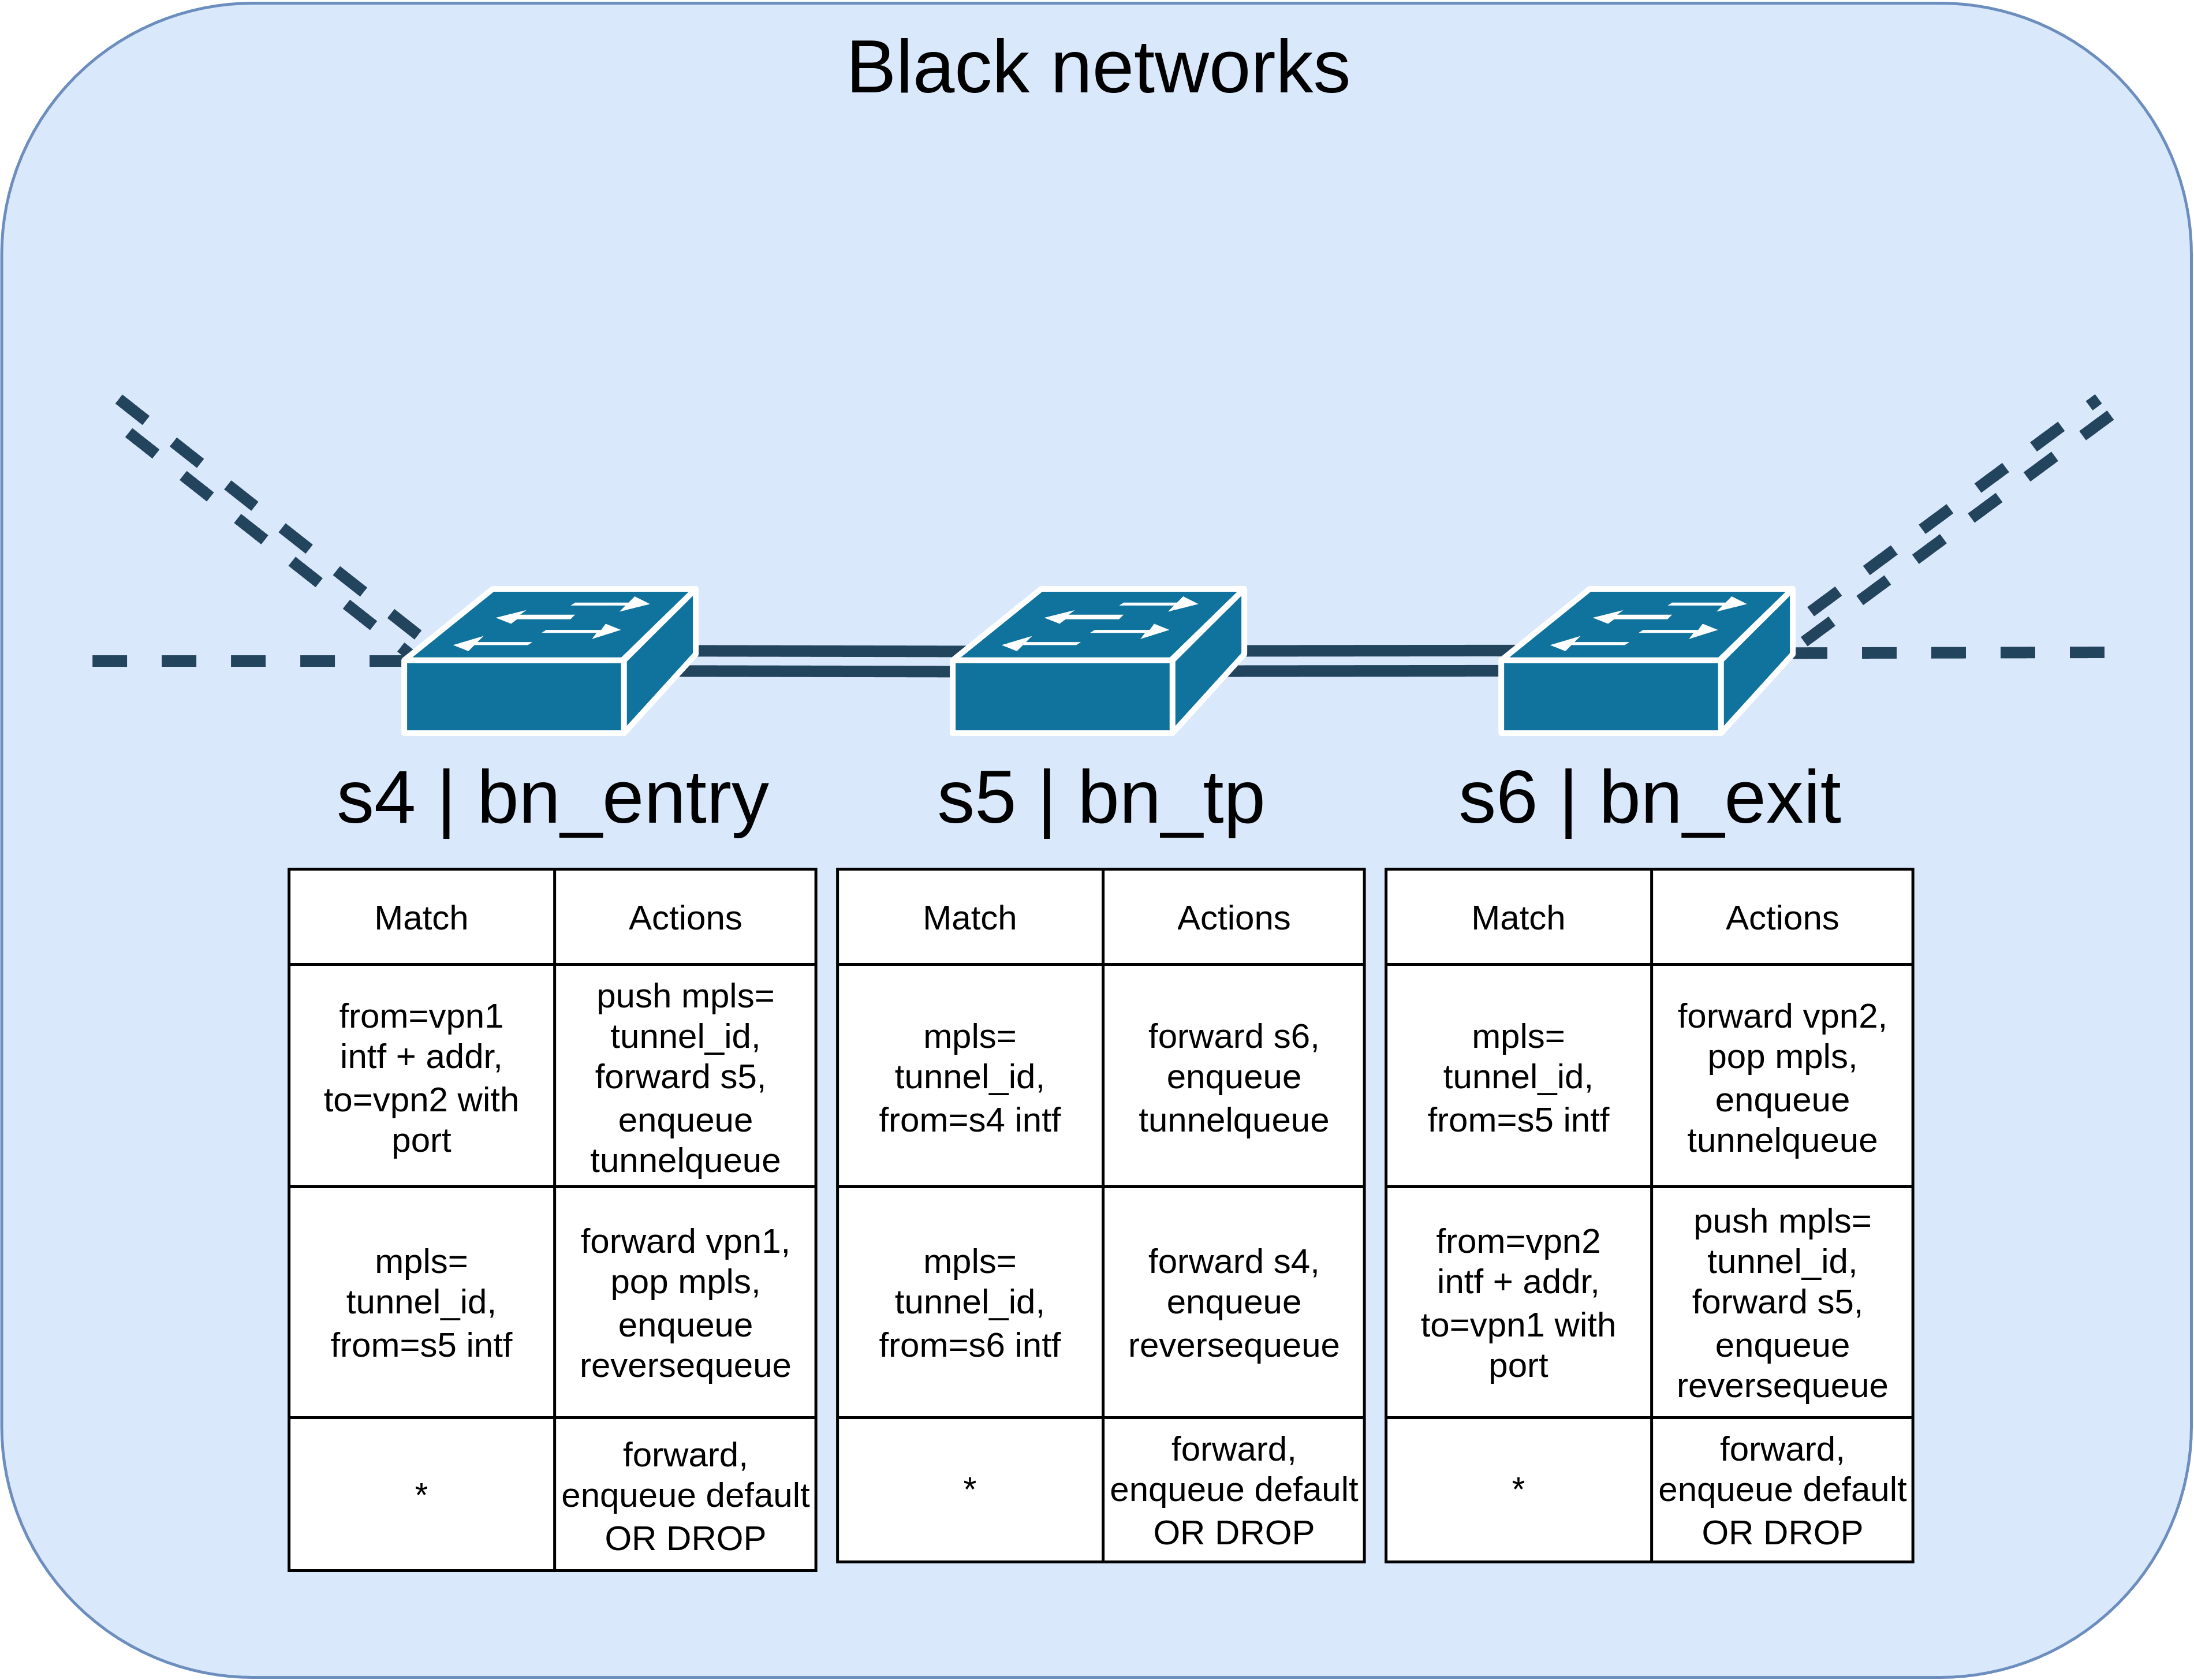
\includegraphics[width=8cm]{images/chapter_6/routing_bn.png}
    \caption[Routing on the \gls{blacknetwork}s]{The routing rules on the \gls{blacknetwork}s for the switches according to their roles. The dotted lines to the left lead to the source \gls{edgenetwork} and the dotted lines on the right lead to the destination \gls{edgenetwork}.}
    \label{fig:routing_bn}
\end{figure}

Afterwards we will establish the following rules depending on the role (see Figure \ref{fig:routing_bn}):

\paragraph{BN\_ALL} We will match all packets from both directions on the correct ingress interface for the \acrshort{udp} destination port and destination address. We will then forward traffic.

\paragraph{BN\_ENTRY} We will match all packets from the main direction on the correct ingress interface for the \acrshort{udp} destination port and IP destination address. We will then tag the packet with the tunnel ID as \acrshort{mpls} label and forward traffic.

For reverse traffic we will match for the tunnel ID \acrshort{mpls} label on the correct ingress interface. We will then remove the tunnel ID \acrshort{mpls} label and forward the traffic.

\paragraph{BN\_TP} We will match all packets from both directions on the correct ingress interface and for the tunnel ID \acrshort{mpls} label. We then forward traffic to the next hop, including the \acrshort{mpls} label.

\paragraph{BN\_EXIT} This switch will receive the reverse rules from \textit{BN\_ENTRY}. It will thus match for the tunnel ID \acrshort{mpls} label on the correct ingress interface, pop the \acrshort{mpls} label and forward the traffic to the \acrshort{vpn} gateway tunnel exit.

For the reverse direction it will match for the correct ingress interface, \acrshort{udp} port and IP destination address, before tagging the packet with the tunnel ID \acrshort{mpls} label and forwarding traffic.

\paragraph{} Concerning the traffic forwarding on a default slice, the same applies as with the source and destination \gls{edgenetwork}s. Please note however that the \acrshort{vpn} gateways will never forward any traffic. Therefore, routing of a default slice (when configured manually) has to be routed around the \acrshort{vpn} gateways, for example by using a different link between a \textit{SRC\_EXIT} and \textit{BN\_ENTRY} switch (or other valid combinations).


\section{Lessons learned}
Of course we encountered some issues while implementing our solution. We will discuss them here and present their solution, so that future developers will not face the same issues. We will begin with MTU considerations and \acrshort{mpls} label popping in \Gls{openflow}, before presenting checksum offloading issues and write queue overflows in the linux kernel.

%\cgn{Maybe instead of Challenges, change the heading to Lessons learned. Challenges sound like unsolved problems. However, in this case you faced issues and had solutions for those.}

\subsection{MTU considerations}
Maybe one of the most obvious issues are MTU considerations. Our multiple \acrshort{mpls} and \acrshort{gre}TAP headers (see Figure \ref{fig:packet_structure}) will attach information to packets, alongside the additional encapsulation by \gls{wireguard}. When packets get close to the network MTU in size, this can lead to fragmentation of packets that would otherwise fit in the MTU. In our case, packets would no longer be delivered after being fragmented. To combat this, a lower MTU than the network MTU should be applied on the hosts. We chose 1300 in our host \acrshort{lxc} container image, which is 200 byte smaller than the network MTU. Slightly higher values might be possible, but this has not been investigated.

\begin{figure}[hp]
    \centering
    \includegraphics[width=10cm]{images/chapter_6/packet_structure.png}
    \caption[Additional headers of packets]{This figure shows the additional headers that a packet receives while traveling through our architecture according to the routing rules specified in Section \ref{impl_concepts}. These additional headers decrease our MTU for packets that we can accept. Our payload is in white, layer two to four headers in red and \acrshort{mpls} headers are in blue. Gray is used to indicate encrypted content within the \gls{wireguard} tunnel, acting as a payload for the tunnel.}
    \label{fig:packet_structure}
\end{figure}

\subsection{MPLS label popping in OpenFlow}
Headaches have been caused due to the \acrshort{mpls} label popping implemented in \Gls{openflow}. The author assumed, that when popping an \acrshort{mpls} label, one has to submit the \acrshort{mpls} label ID that should be popped. This would make sense because it is possible to stack multiple \acrshort{mpls} labels and maybe the second or third in the stack should get popped. This is however not the case. Instead one has to specify the \gls{ethertype} of the resulting packet \cite{openflow}, which would be 2048 (or 0x800) for \acrshort{ipv4} \cite{rfc7042}. This caused corrupt packets on the destination host.

\subsection{Checksum offloading issues}
Another issue with corrupt packets on the destination host was caused by invalid \acrshort{udp} and \acrshort{tcp} checksums. When pushing or popping \acrshort{mpls} labels, current implementations of \Gls{ovs} break the \acrshort{udp} and \acrshort{tcp} checksums while \acrshort{tx} (write) offloading is enabled on the switch interfaces. To fix the checksum calculations, one has to disable \acrshort{tx} offloading on all switch interfaces like this:

\begin{lstlisting}[language=bash]
ethtool --offload $INTF_NAME tx off
\end{lstlisting}

More information on this can be found in the linux kernel documentation \cite{txoffload}.

\subsection{Write queue overflow}
While testing our slicing architecture under a flooding attack locally, we noticed that packets were being dropped on the \acrshort{vpn} gateway. We decided to investigate this in more detail, because traffic from the adversaries was not even flowing through the \acrshort{vpn} gateways, but would rather flow around them (as described in Section \ref{impl_tunnel_config}). This was very unexpected for us in the beginning. We noticed that packets were received by the \acrshort{vpn} gateway, but were dropped on the tunnel interface before entering the \gls{wireguard} tunnel.

Our first measure was to increase the \acrshort{tx} (write) queue size, which improved the result but still saw dropped packets. After trying some other approaches which all failed to solve the problem, we finally found the solution.

By pinning the adversaries to certain CPU threads that they can use, the \acrshort{tx} queue would no longer overflow. It was interesting that we could even pin the attackers to all but one thread to stop packets from dropping. We currently assume that this happens due to CPU spikes caused by the adversaries while using \textit{hping3}, which stole enough computational time from the \acrshort{vpn} gateways to make them drop packets.

Subsequently we stuck to the CPU pinning of the attackers, but still assigned all but one or two threads to them which should have next to negligible impact and is more than generous (30 out of 32 threads and 3 out of 4 threads in our tests). This is also a realistic approach, as usually in a real-world network, attackers would not share the same CPU with our switches or \acrshort{vpn} gateways. However this may not always be the case in container setups. An easy solution to this could be to apply resource limits to containers as is common practice in modern setups.
